%%%%%%%%%%%%%%%%%%%%%%%%%%%%%%%%%%%%%%%%%%%%%%%%%%%%%%%%%%%%%%%%%%%%%%%%
%                                                                      %
%     File: Thesis_Conclusions.tex                                     %
%     Tex Master: Thesis.tex                                           %
%                                                                      %
%     Author: Andre C. Marta                                           %
%     Last modified :  2 Jul 2015                                      %
%                                                                      %
%%%%%%%%%%%%%%%%%%%%%%%%%%%%%%%%%%%%%%%%%%%%%%%%%%%%%%%%%%%%%%%%%%%%%%%%

\chapter{Analysis}
\label{chapter:analysis}

\section{Overview of the $hh\rightarrow b\overline{b}b\overline{b}$ channel}
- Signal cross section and final state signature \\
- Pros and challenges of using the 4b final state \\
- Main backgrounds (the ones we consider) and respective cross sections (leave for appendix discussion on other backgrounds, namely Higgs processes)\\
----------------------------------------------------------------\\
\begin{figure}
	\centering
	\begin{minipage}{.45\textwidth}
		\centering
		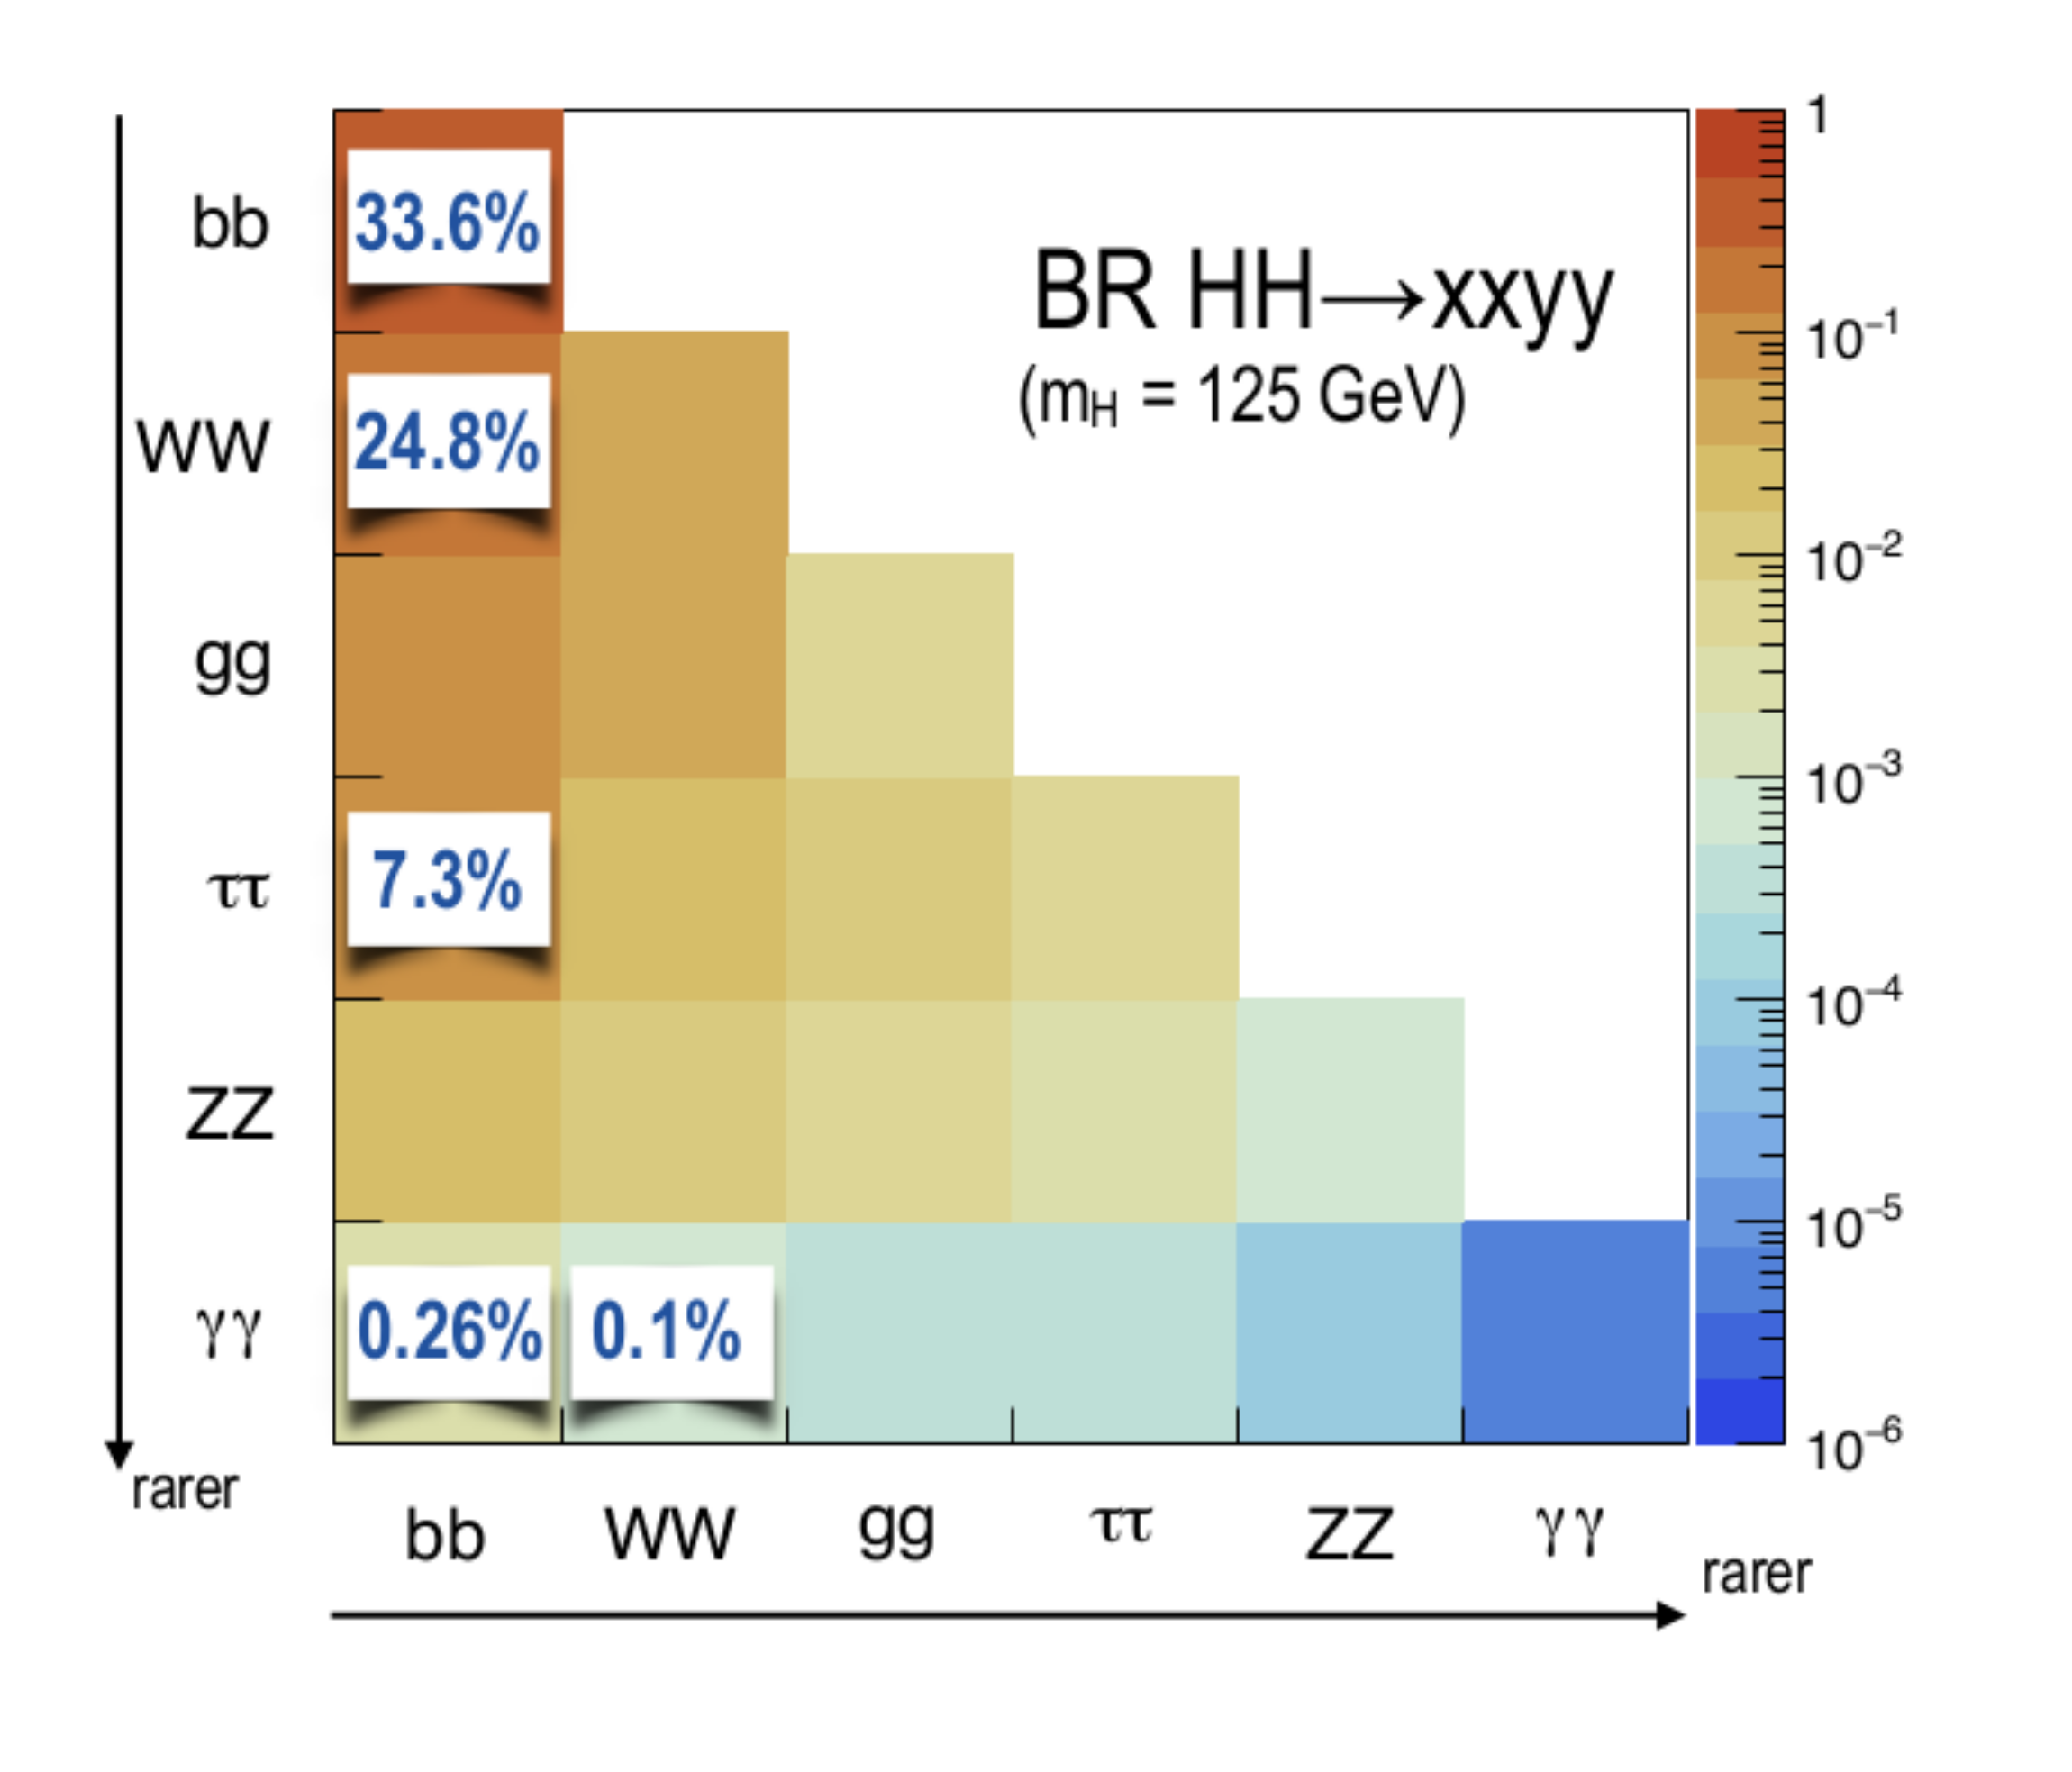
\includegraphics[width=\linewidth]{./Figures/hhBR.png}
		\caption{Higgs pairs branching ratios.}
		\label{fig_hhBR}
	\end{minipage}%
	\begin{minipage}{.55\textwidth}
		\centering
		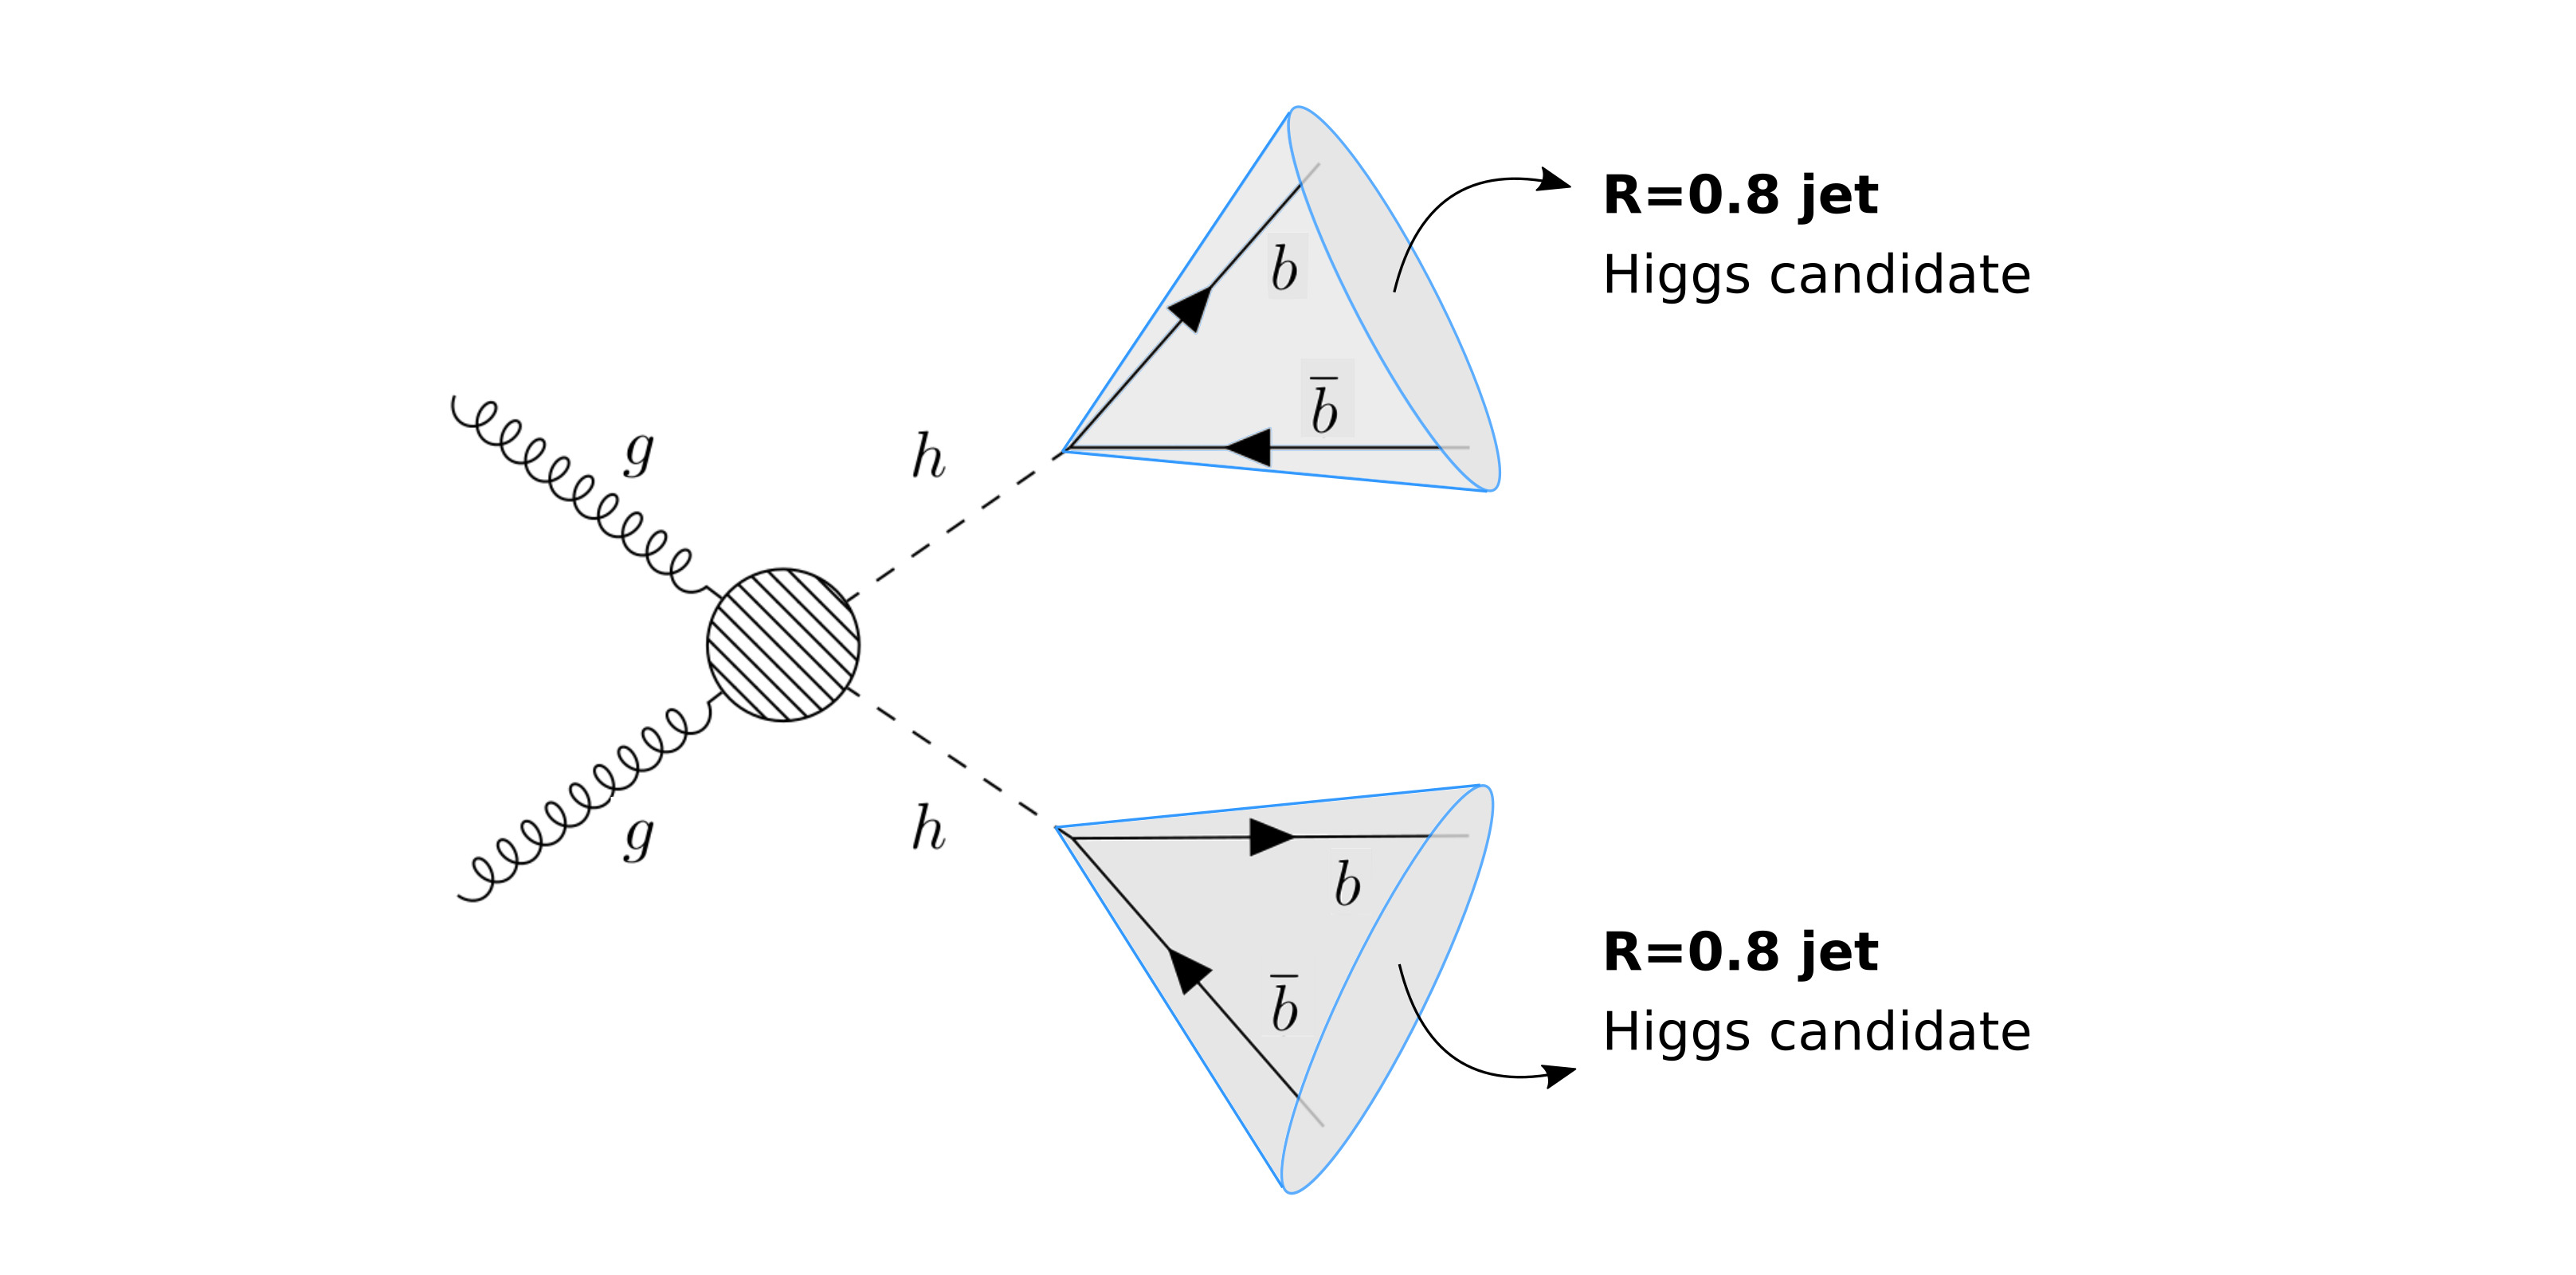
\includegraphics[trim={4cm 0 5cm 0},clip,width=\linewidth]{./Figures/boosted1.png}
		\caption{Event topology targeted by the boosted analysis region. The blob represents the interaction between the gluons and the Higg bosons that is represented by the Feynman diagrams shown in figure \ref{fig:higgs_pair}.}
		\label{fig:final_state}
	\end{minipage}
	\label{fig:boosted}
\end{figure}

%\begin{figure}
%	\centering
%	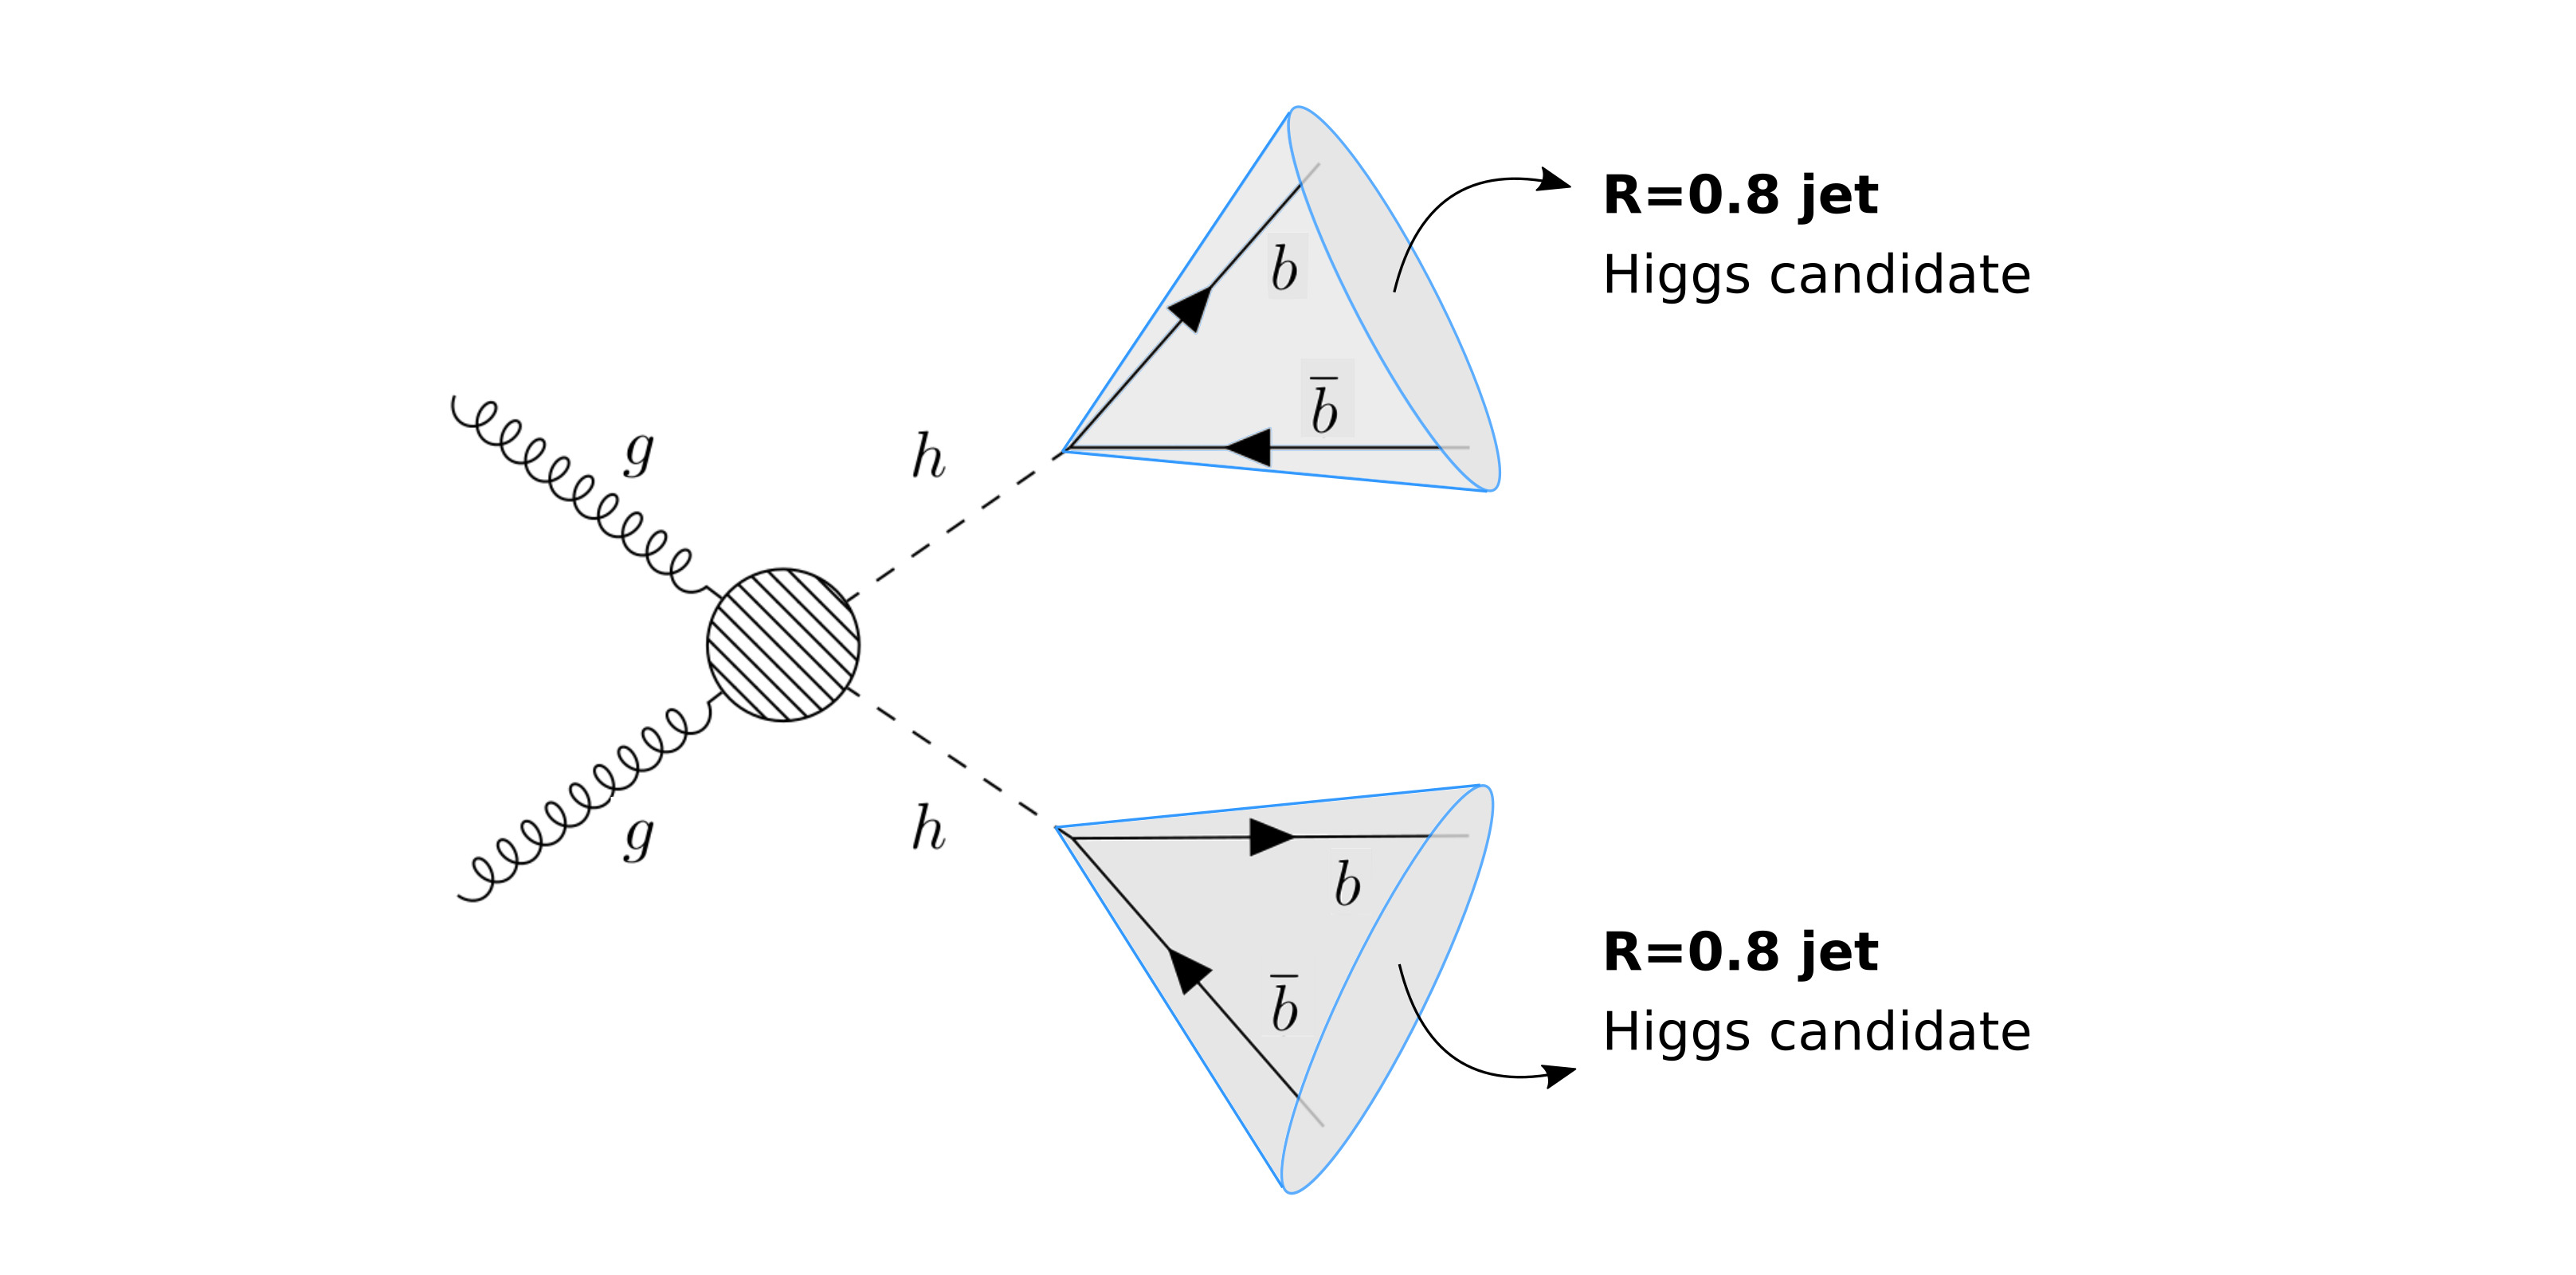
\includegraphics[width=\textwidth]{./Figures/boosted1.png}
%	%\hfill
%	%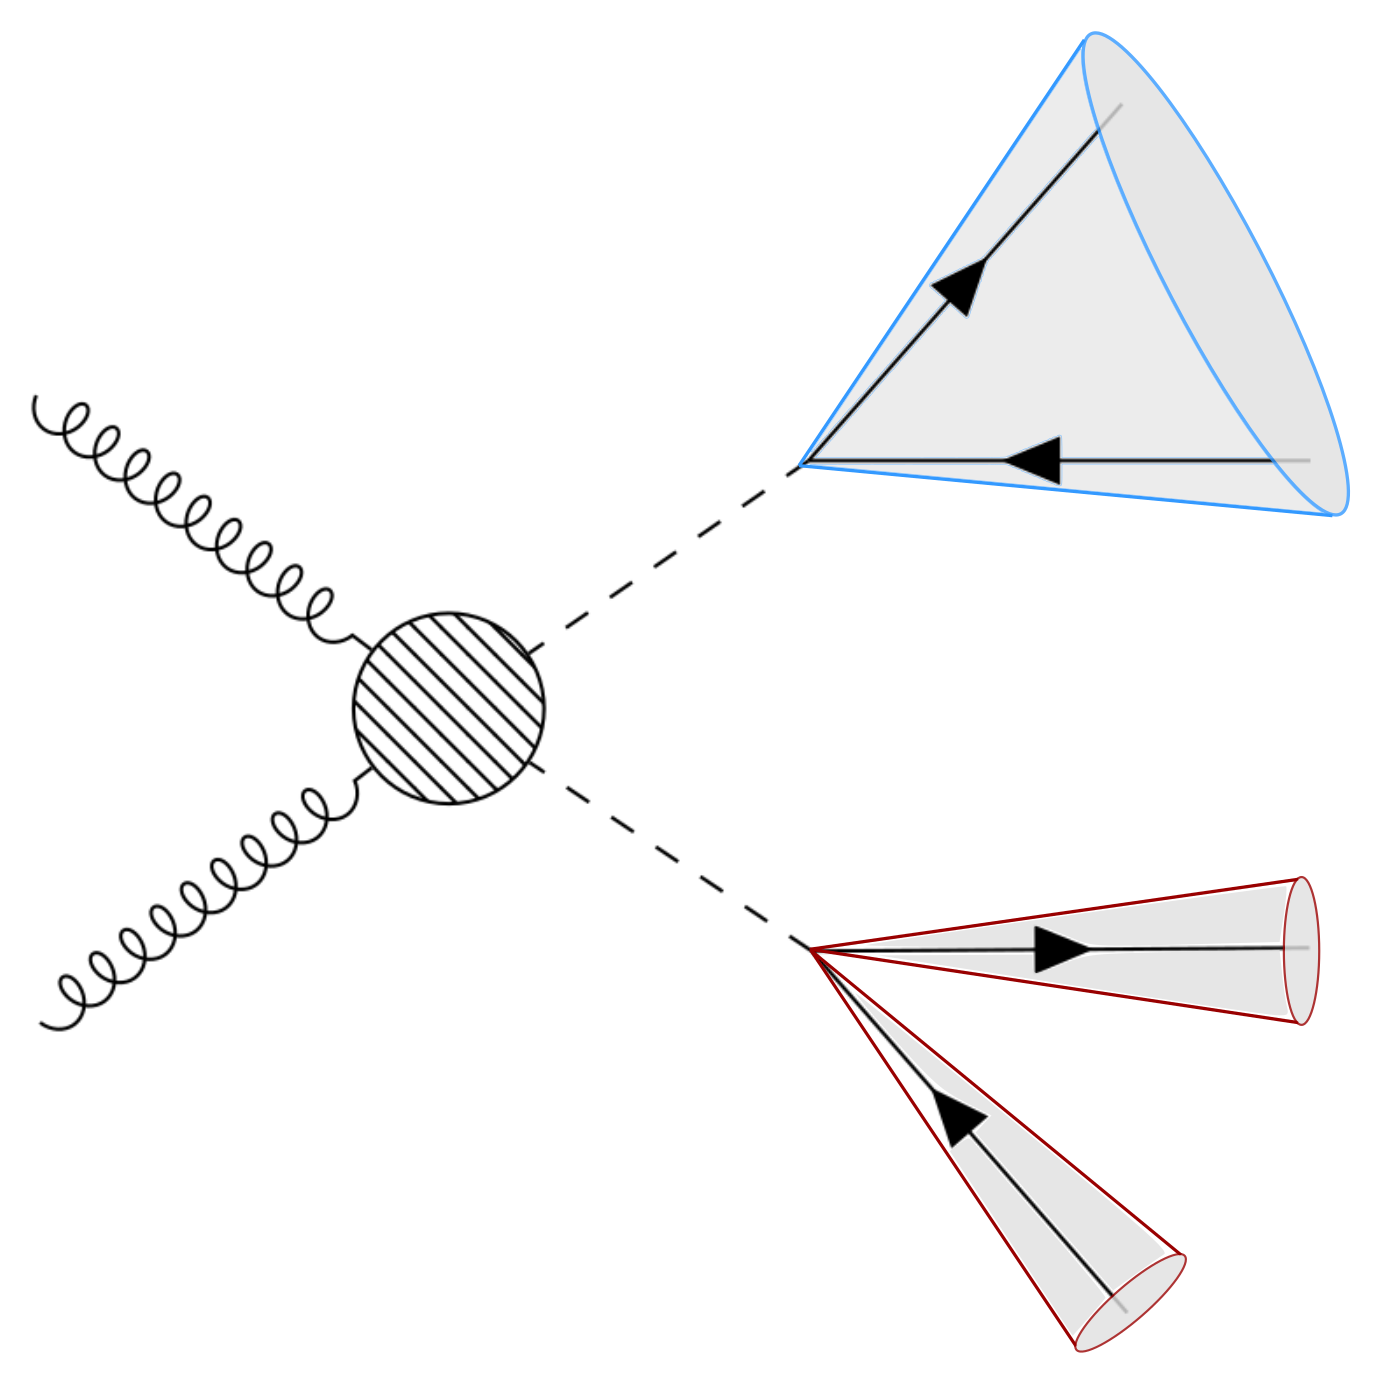
\includegraphics[width=.45\textwidth]{./Figures/inter.png}
%	\caption{Event topology targeted by the boosted analysis region. The blob represents the interaction between the gluons and the Higg bosons that is represented by the Feynman diagrams shown in figure \ref{fig:higgs_pair}.}
%	\label{fig:final_state}
%\end{figure}
%
%\begin{figure}
%	\centering
%	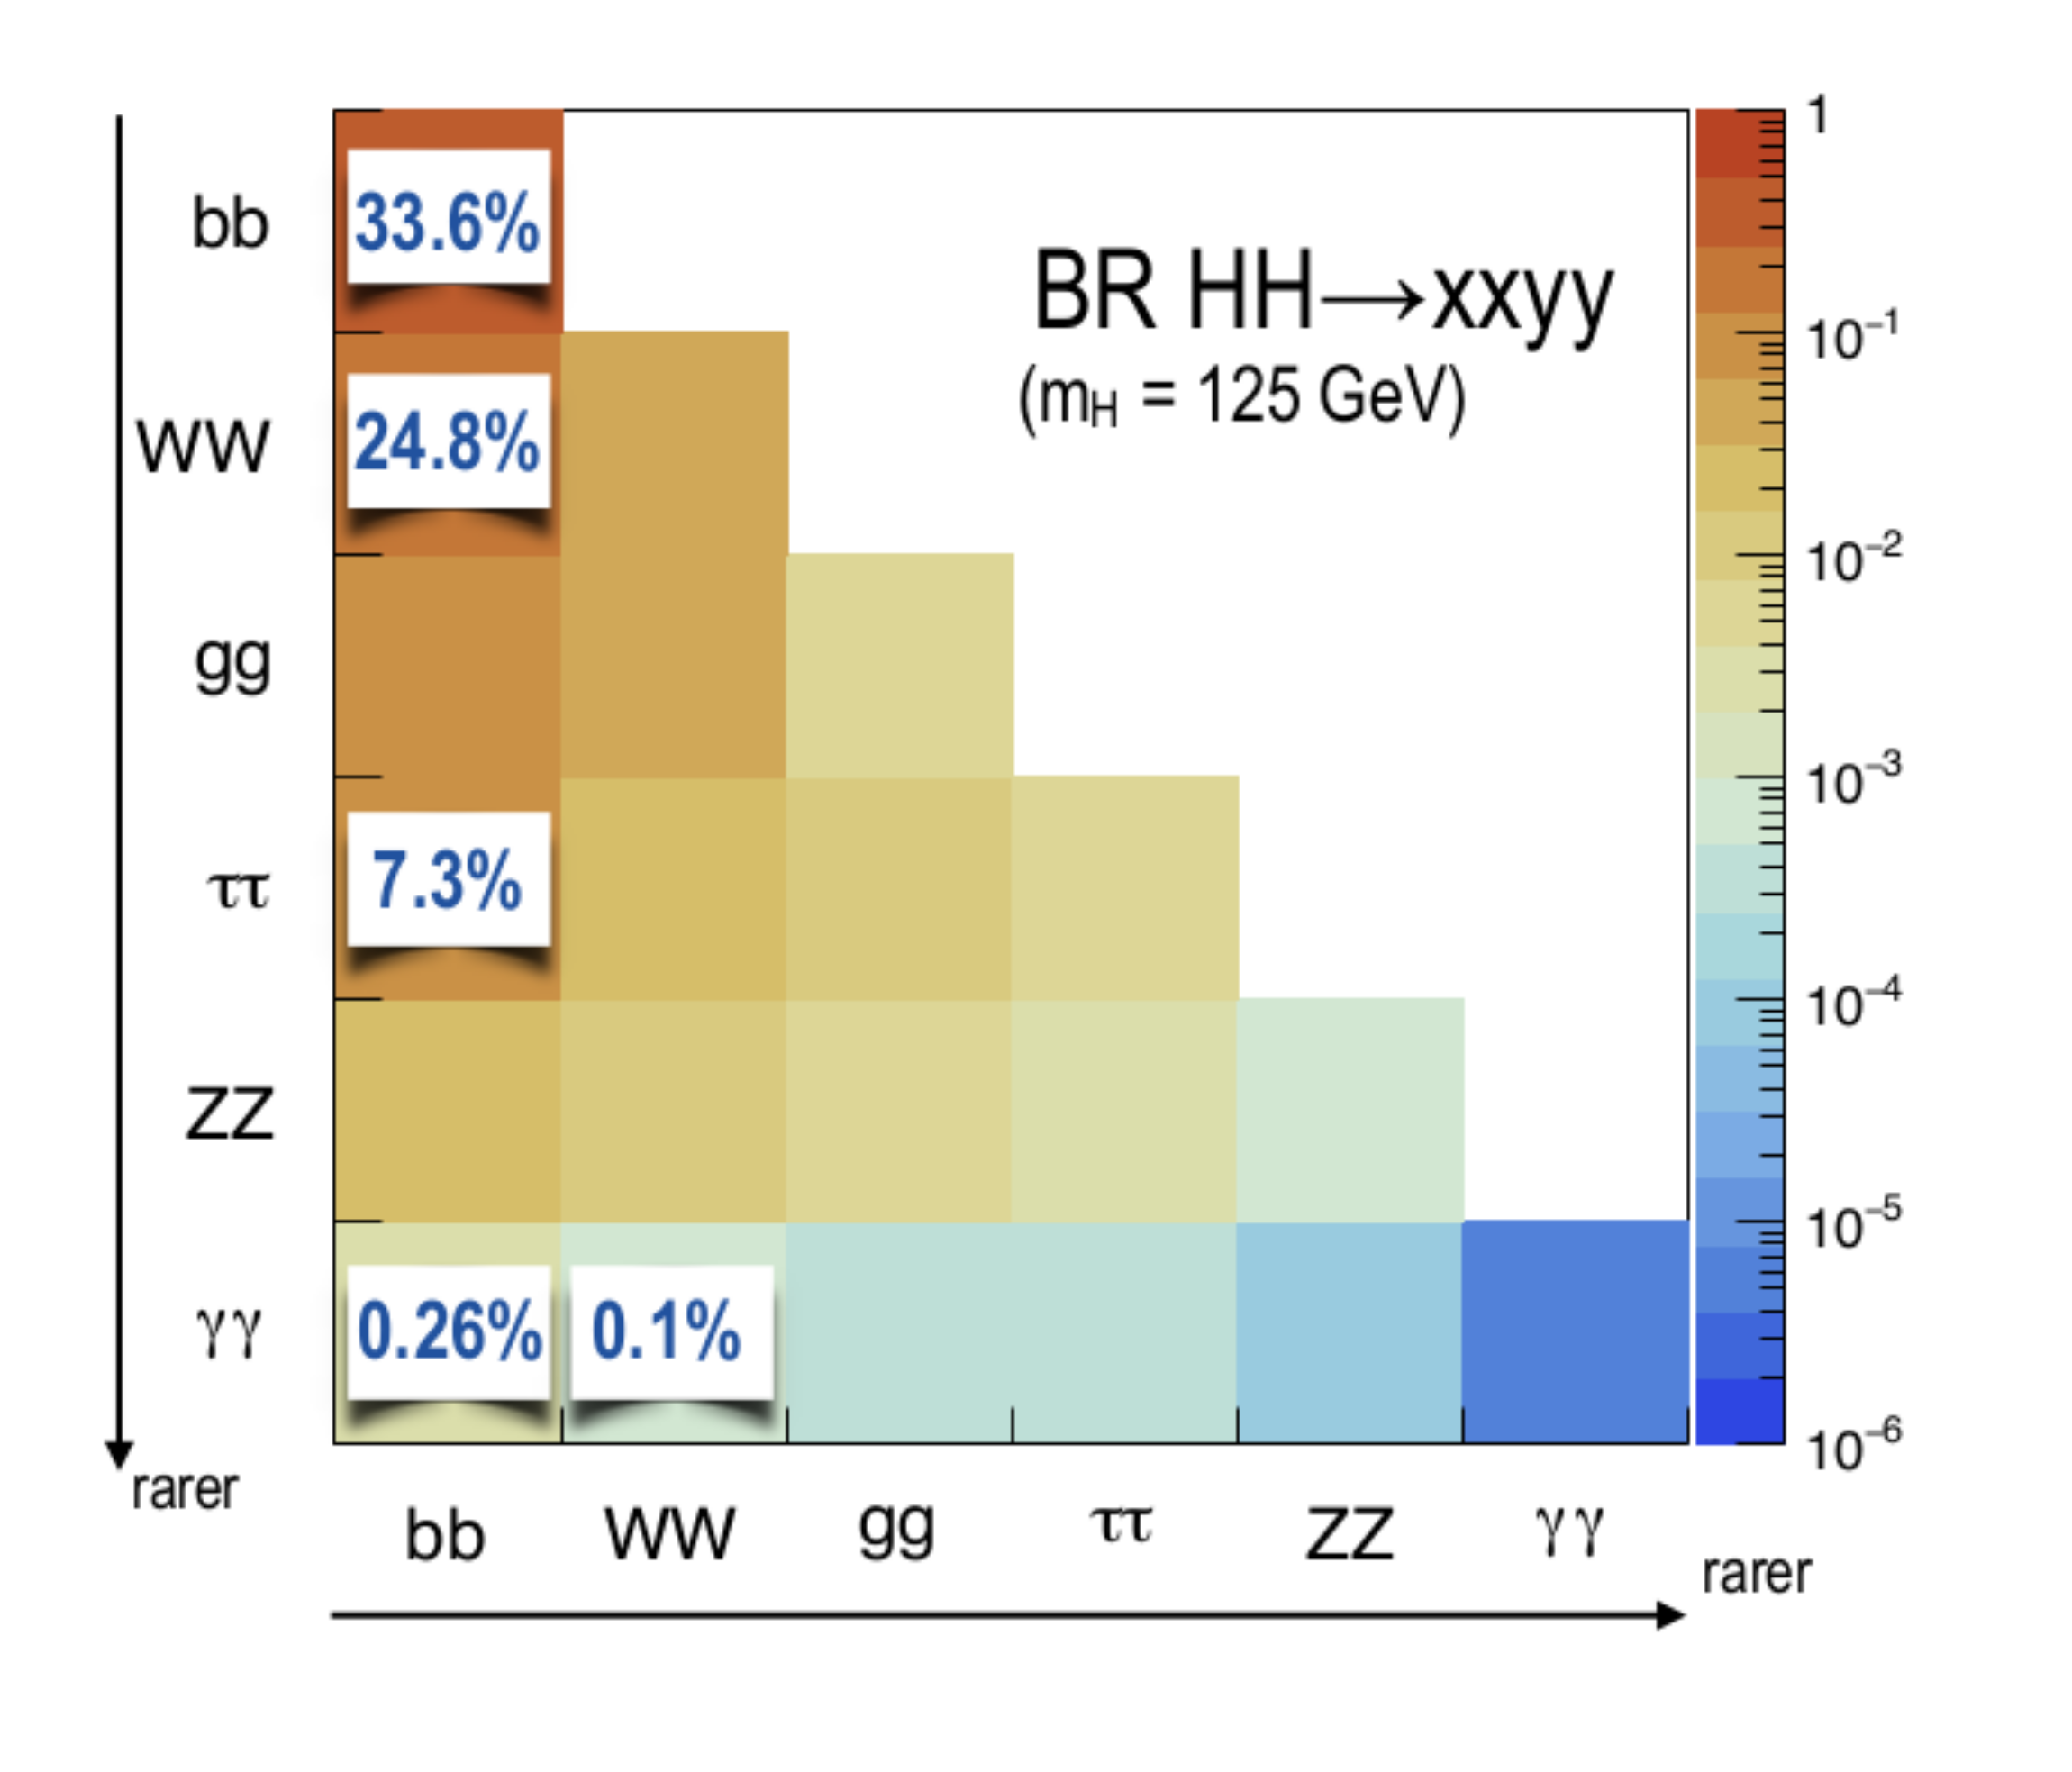
\includegraphics[width=0.6\textwidth]{./Figures/hhBR.png}
%	\label{fig:hhBR}
%	\caption{Higgs pair branching ratios.}
%\end{figure}

The searches for Higgs pair production in the four b quarks final state benefit from the large BR of $h\rightarrow b\overline{b}$. For the SM Higgs, with a mass around $125$ GeV, the branching ratio of the $hh\rightarrow b\overline{b}b\overline{b}$ decay is approximately $33.6\%$, making it the most probable decay for Higgs pairs, as it is illustrate in Figure \ref{fig:hhBR}.

%This leads to a cross section times BR of $\sim 0.7$ pb. 

However, in this channel, the main background is QCD multijet production that has a cross section several orders of magnitude larger than di-Higgs production in the SM, as Table \ref{table:samples_summary} shows. Nonetheless, it is a well known feature of QCD that the majority of jets produced are soft. This means that the $p_T$ distributions of this background have a very large yield close to zero and then fall very steeply while the signal has a much larger tail to high values of $p_T$. This indicates that searches targeting the boosted kinematic regime may be the key to measure $hh\rightarrow b\overline{b}b\overline{b}$ using inclusive production.

In this work we target the boosted regime. In this kinematic region, the final state of the signal is characterized by two jets with a large R parameter. Each jet is expected to contain the two b quarks originated from the decay of a Higgs boson, as Figure \ref{fig:final_state} illustrates. Extra jets are also expected to be reconstructed as a consequence of QCD activity. 

The analysis presented here is performed using the Monte-Carlo samples described in chapter \ref{chapter:tools}. All samples assume $m_h=125$ GeV. The event selection criteria are designed to optimize the significance, given by $S/\sqrt{B}$, where $S$ and $B$ represent the number of signal and background events, respectively. 

%In addition, the jets produced by QCD interaction are more likely to be initiated by a gluon or a light quark. Therefore, tight b-tagging criteria and algorithms based on substructure variables can also help reject this background. 

\subsection{Event pre-selection}

TO INCLUDE: \\
- discussion on trigger requirements: important in real analysis\\
- show and discuss some distributions: invariant mass (h, hh), momentum, tau21, delta eta (hh), more substructure variables (may be all that we considered relevant)\\
- compare with other articles/analysis ? \\

--------------------------------------------------------------------------------------------------\\
We start by applying very simple and loose cuts that target events consistent with the boosted topology. 

We require at least two b-tagged $R=0.8$ jets (which corresponds to at least four b-tagged subjets, at least two in each $R=0.8$ jet). In addition, the leading and sub leading jets must have $p_T\geq200$ GeV in order for the event to be accepted. From equation \ref{eq:deltaR}, a Higgs boson with $p_T=200$ GeV leads to a pair of b quarks with $\Delta R\sim \frac{2m}{p_T}=1.25$. Therefore, considering jet with $R=0.8$ (diameter equal to $1.6$) and $p_T\geq 200$ is a reasonable choice. For a more complete description about the jet radius see appendix \ref{chapter:jetrad}. Due to the b-tagging efficiency formulas (that are described in detail in section \ref{sec:btagging}), there is a natural cutoff at $|\eta|=4$ so we do not place any additional cut in $\eta$. From now on, these cuts are referred to as pre-selection cuts.

After the pre-selection cuts we can plot all the relevant distributions that allow us to characterize the signal and background events. These are shown in the next two sections. In addition, these distributions provide a first insight into the discriminating power of the kinematic and substructure variables that are explored.  

\subsection{Signal characterization}

The cross section for di-Higgs inclusive production from $pp$ collisions at $100$ TeV is $1.2$ pb \cite{FCCphys}. This value is computed at NLO accuracy. The dominant process is gluon-gluon fusion that has been extensively discussed in section \ref{section:Higgs_pair}. The signal process comprehends the di-Higgs inclusive production and the $hh\rightarrow b\overline{b}b\overline{b}$ subsequent decays. The total process cross section is then given by $\sigma(pp\rightarrow hh)\times BR(hh\rightarrow b\overline{b}b\overline{b})$ and it amounts to approximately $0.4$ pb [NOT VERY COHERENT WITH MG VALUES - CHECK]. For an integrated luminosity of $3000\text{fb}^{-1}$ of proton collisions at $\sqrt{s}=100$ TeV we expect X events.

The Higgs candidates are reconstructed using large R jets that can be directly measured using information from the calorimeters and tracking systems. Figure \ref{fig:hh_deltaPhi} shows the $\Delta\phi$ between the two leading jets (Higgs candidates), $\Delta\phi(hh)$. For a large fraction of the signal events (red curve) $\Delta\phi(hh)\sim \pi$ which indicates that the jets are produced back-to-back in the transverse plane. There is also a small fraction of events for which the jets have $\Delta\phi(hh)\sim 1$. For these events there must be at least a third jet that balances the momentum of the jets pair. 

Each wide jet is expected to be consistent with having two subjets associated with the two b quarks from the $h\rightarrow b\overline{b}$ decay. In the Higgs rest frame, the two subjets are produced back-to-back conserving momentum. In the laboratory frame, the $\Delta R$ between the subjets depends on the momentum of the Higgs boson, with larger $\Delta R$ corresponding to Higgs bosons with a lower momentum. This correlation between the $\Delta R$ between the subjets of the leading Higgs candidate ($\Delta R(b\overline{b})$) and its momentum ($p_T(h_1)$) is shown in figure \ref{fig:deltaR_bb_pt}. 

The $p_T$ distributions of the leading and sub leading jets (Higgs candidates) are shown in figure \ref{fig:h1h2_pt} on the left and right, respectively. The histograms are normalized to unit area in order to allow for shape comparison between them. For the leading jet the $p_T$ spectrum peaks at approximately $350$ GeV and has a long tail for large values of $p_T$, in particular, longer than any of the backgrounds. For the sub leading jet the spectrum is softer, as expected, but the tail of the distribution is still longer that for any of the backgrounds. These distributions show that the signal process produces jets with a larger transverse momentum than the jets produce by the background processes which indicates that a boosted analysis might perform well.

The $\eta$ distribution of the leading jet is shown in figure \ref{fig:h1_eta_M} on the left. This distribution is limited to $|\eta|<4$ because the b-tagging efficiency goes to zero for $|\eta|>4$ (see section \ref{sec:btagging} for more details). The shape is approximately gaussian which is due to the detector acceptance [EXPLAIN BETTER ?]. The $\eta$ distribution of the sub leading jet is very similar to this one so we abstain from showing it here.

The softdrop mass distribution of the leading jet is shown in figure \ref{fig:h1_eta_M} on the right. For the signal (red curve) there is a clear peak at approximately $120$ GeV which corresponds to the SM Higgs boson mass peak. The peak is quite broad which means the mass resolution in this channel is not very good. On the one hand, this is because we are using large-R jets to reconstruct the Higgs candidates. These objects have a worse mass resolution than other cleaner objects such as photons or electrons.  On the other hand, the cuts applied before plotting these distributions are very loose. As we place additional cut the mass peak can be made slightly narrower. Another interesting feature of the signal's mass spectrum is the existence of a peak close to zero. The explanation is the following. Some jets do not contain both b quarks from the Higgs decay such that when applying the mass drop procedure only one b quark with a mass of approximately $5$ GeV remains inside the jet creating the peak at lower masses. A more detailed discussion, as well as a plot that supports this interpretation, can be found in appendix \ref{chapter:SDmass}.

In addition to the basic kinematic distributions that we just described there are a multitude of other variables one can look at. Here we show the $\Delta\eta$ between the Higgs pairs, figure \ref{fig:hh_deltaEta_h1_tau21} on the left, and the $\tau_{21}$ variable for te leading Higgs candidate, figure \ref{fig:hh_deltaEta_h1_tau21} on the right. The first distribution shows that the Higgs pair tends to have a $\Delta\eta$ very close to zero which indicates that the pair is highly boosted in the longitudinal plane [??]. The $\tau_{21}$ distribution shows that for the signal this variable takes values close to zero which means the jet is consistent with having two subjets.

\begin{figure}
	\centering
	\begin{minipage}{.5\textwidth}
		\centering
		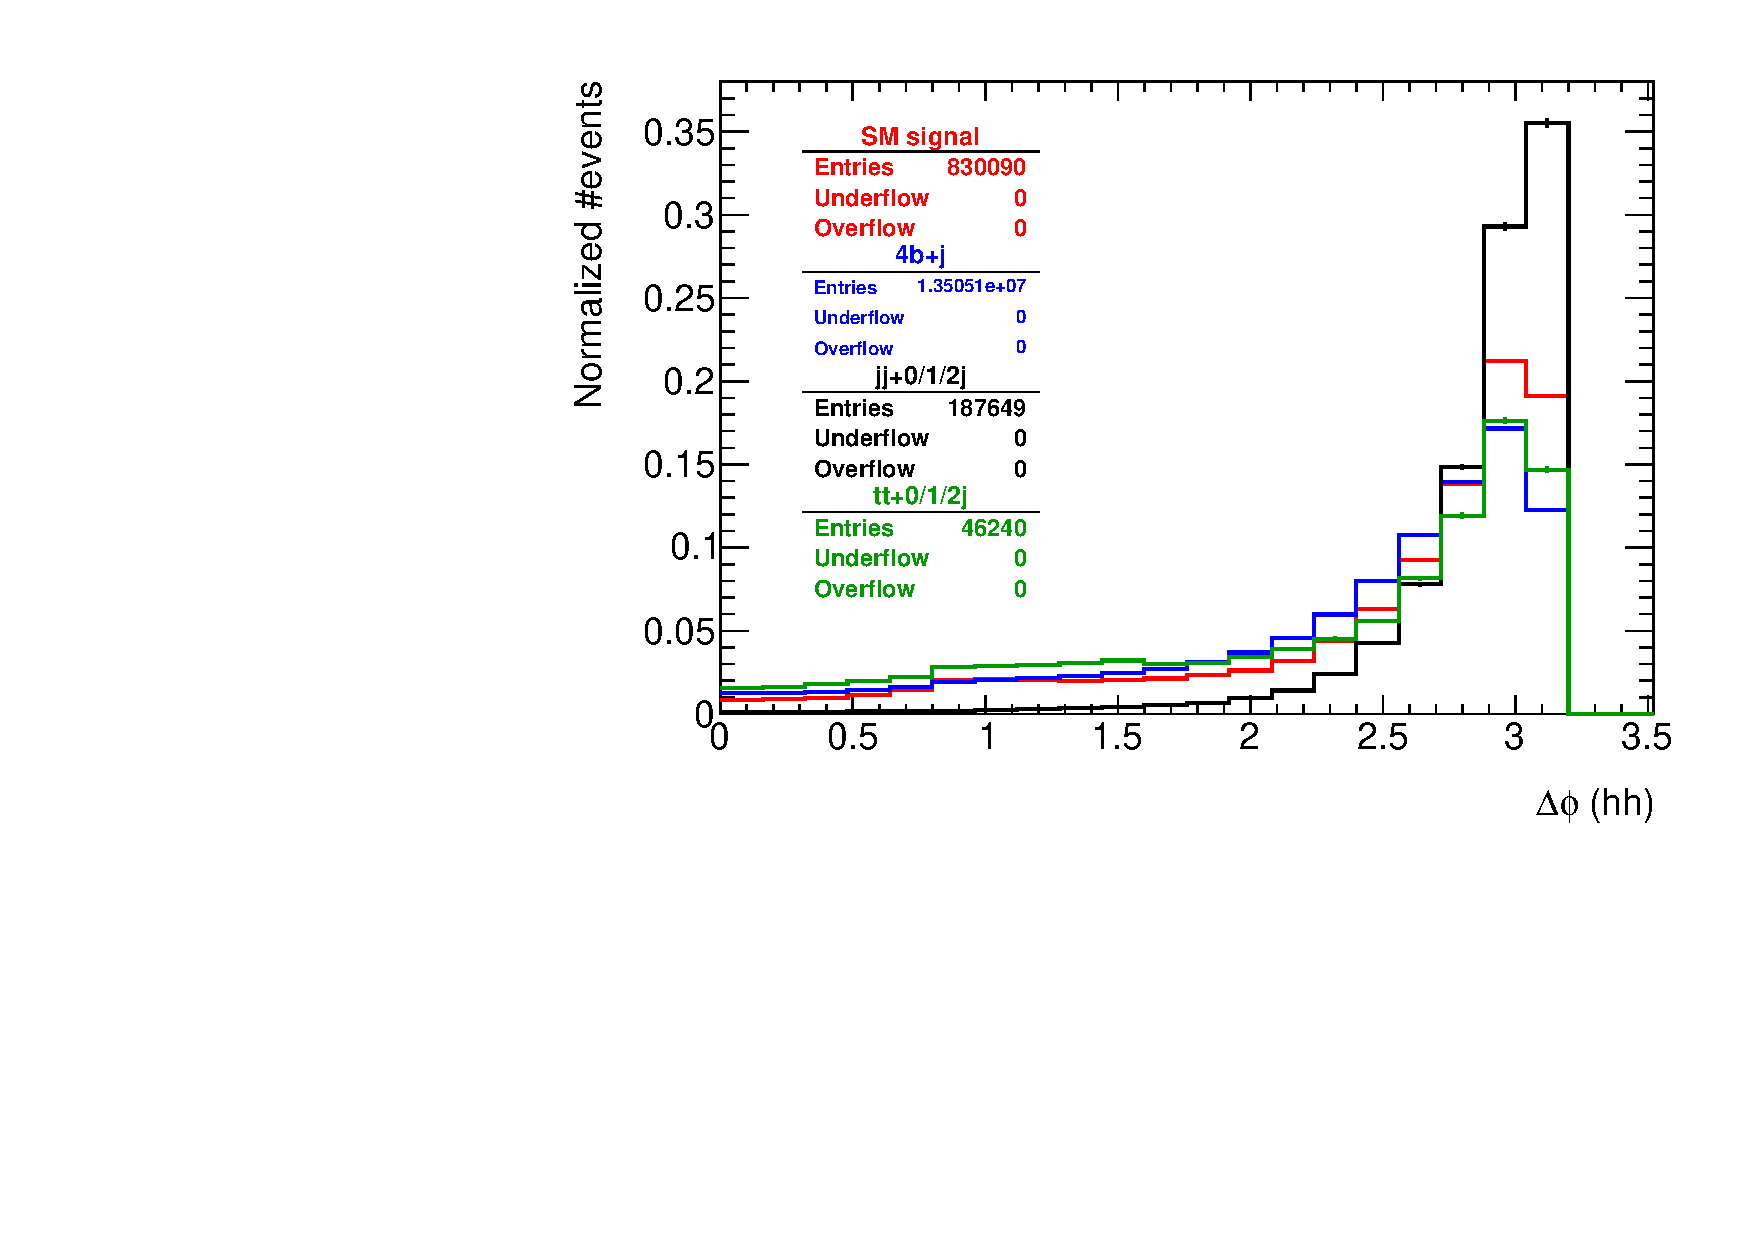
\includegraphics[width=\linewidth]{./Figures/hist_hh_deltaPhi.pdf}
		\caption{$\Delta R$ between the b quarks coming from the decay of the leading Higgs candidate, $h_1$.}
		\label{fig:deltaR_bb_pt}
	\end{minipage}%
	\begin{minipage}{.5\textwidth}
		\centering
		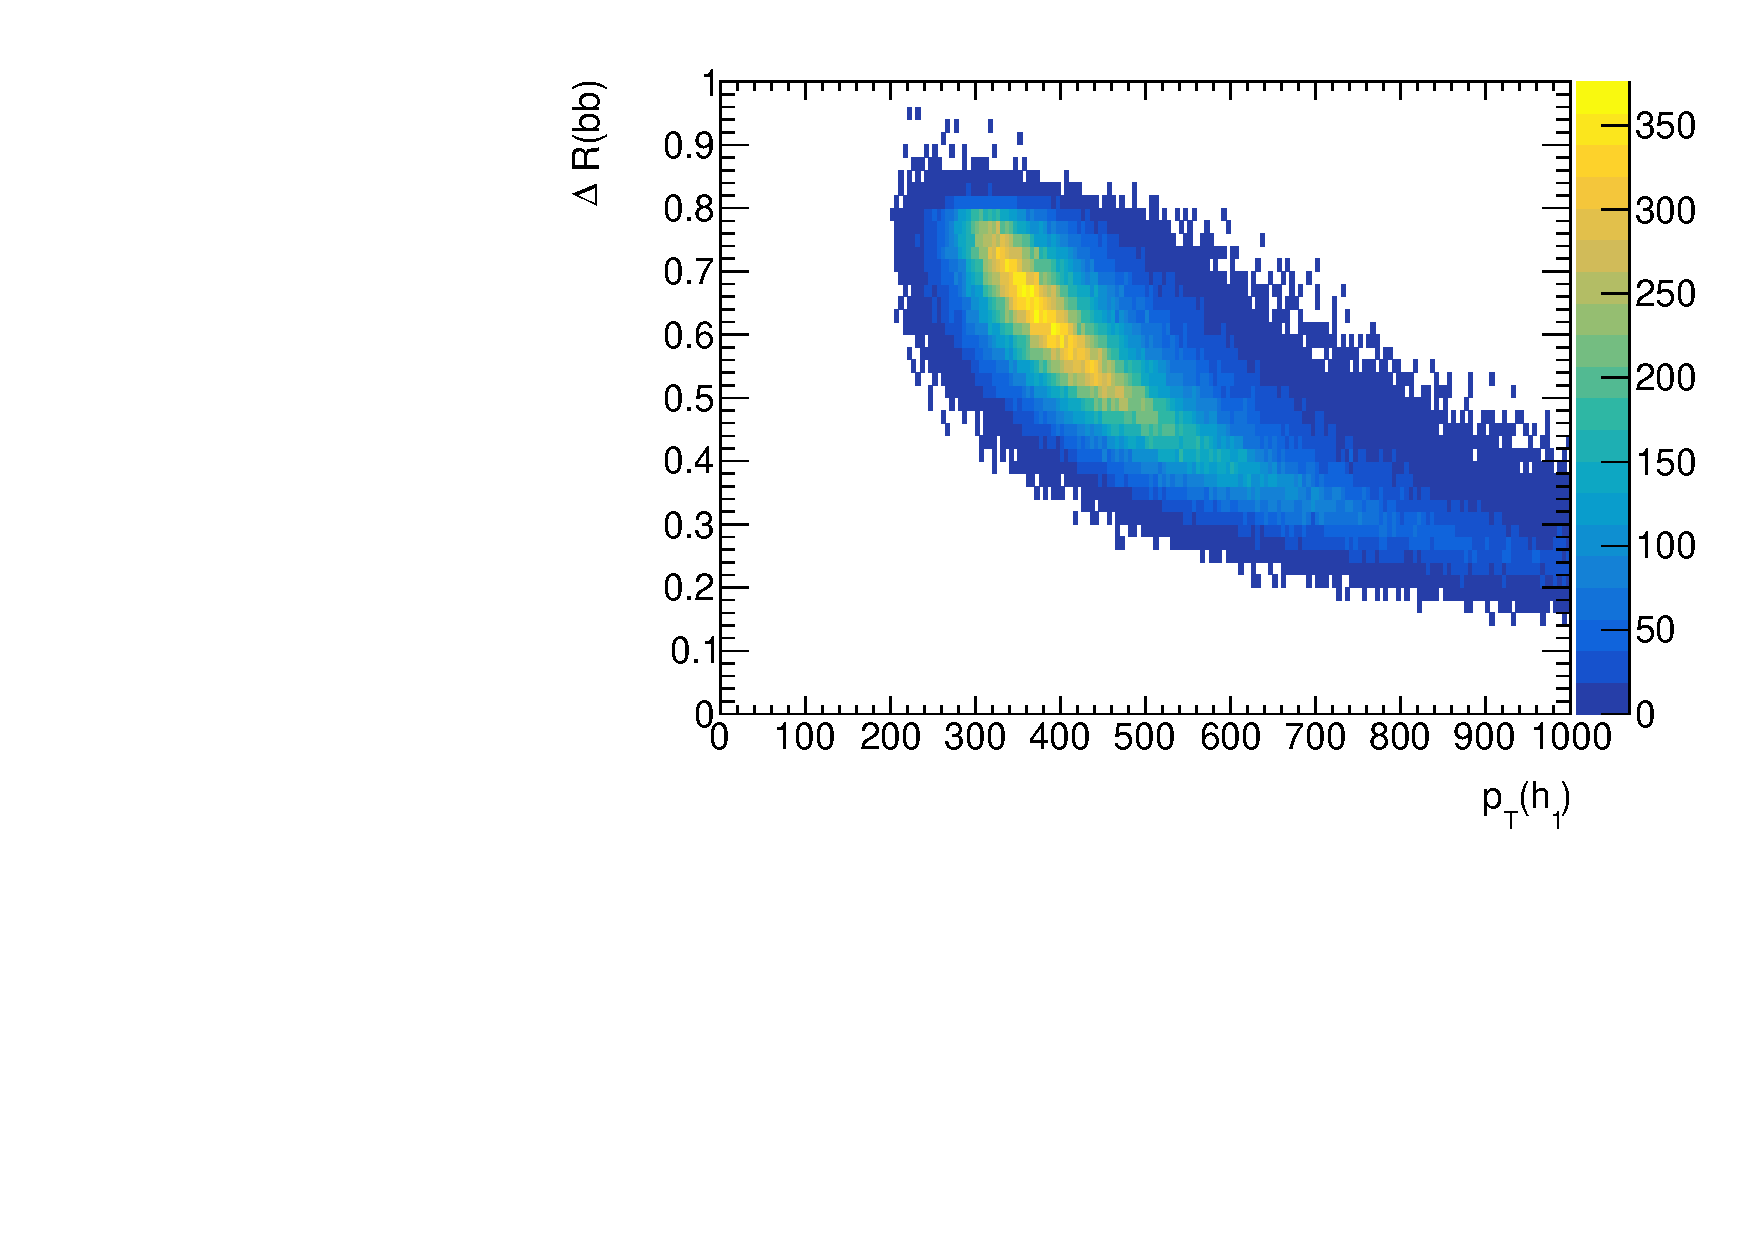
\includegraphics[width=\linewidth]{./Figures/deltaR_bb_pt.pdf}
		\label{fig:hh_deltaPhi}
		\caption{$\Delta\phi$ between the Higgs candidates.}
	\end{minipage}
\end{figure}

%\begin{figure}
%	\centering
%	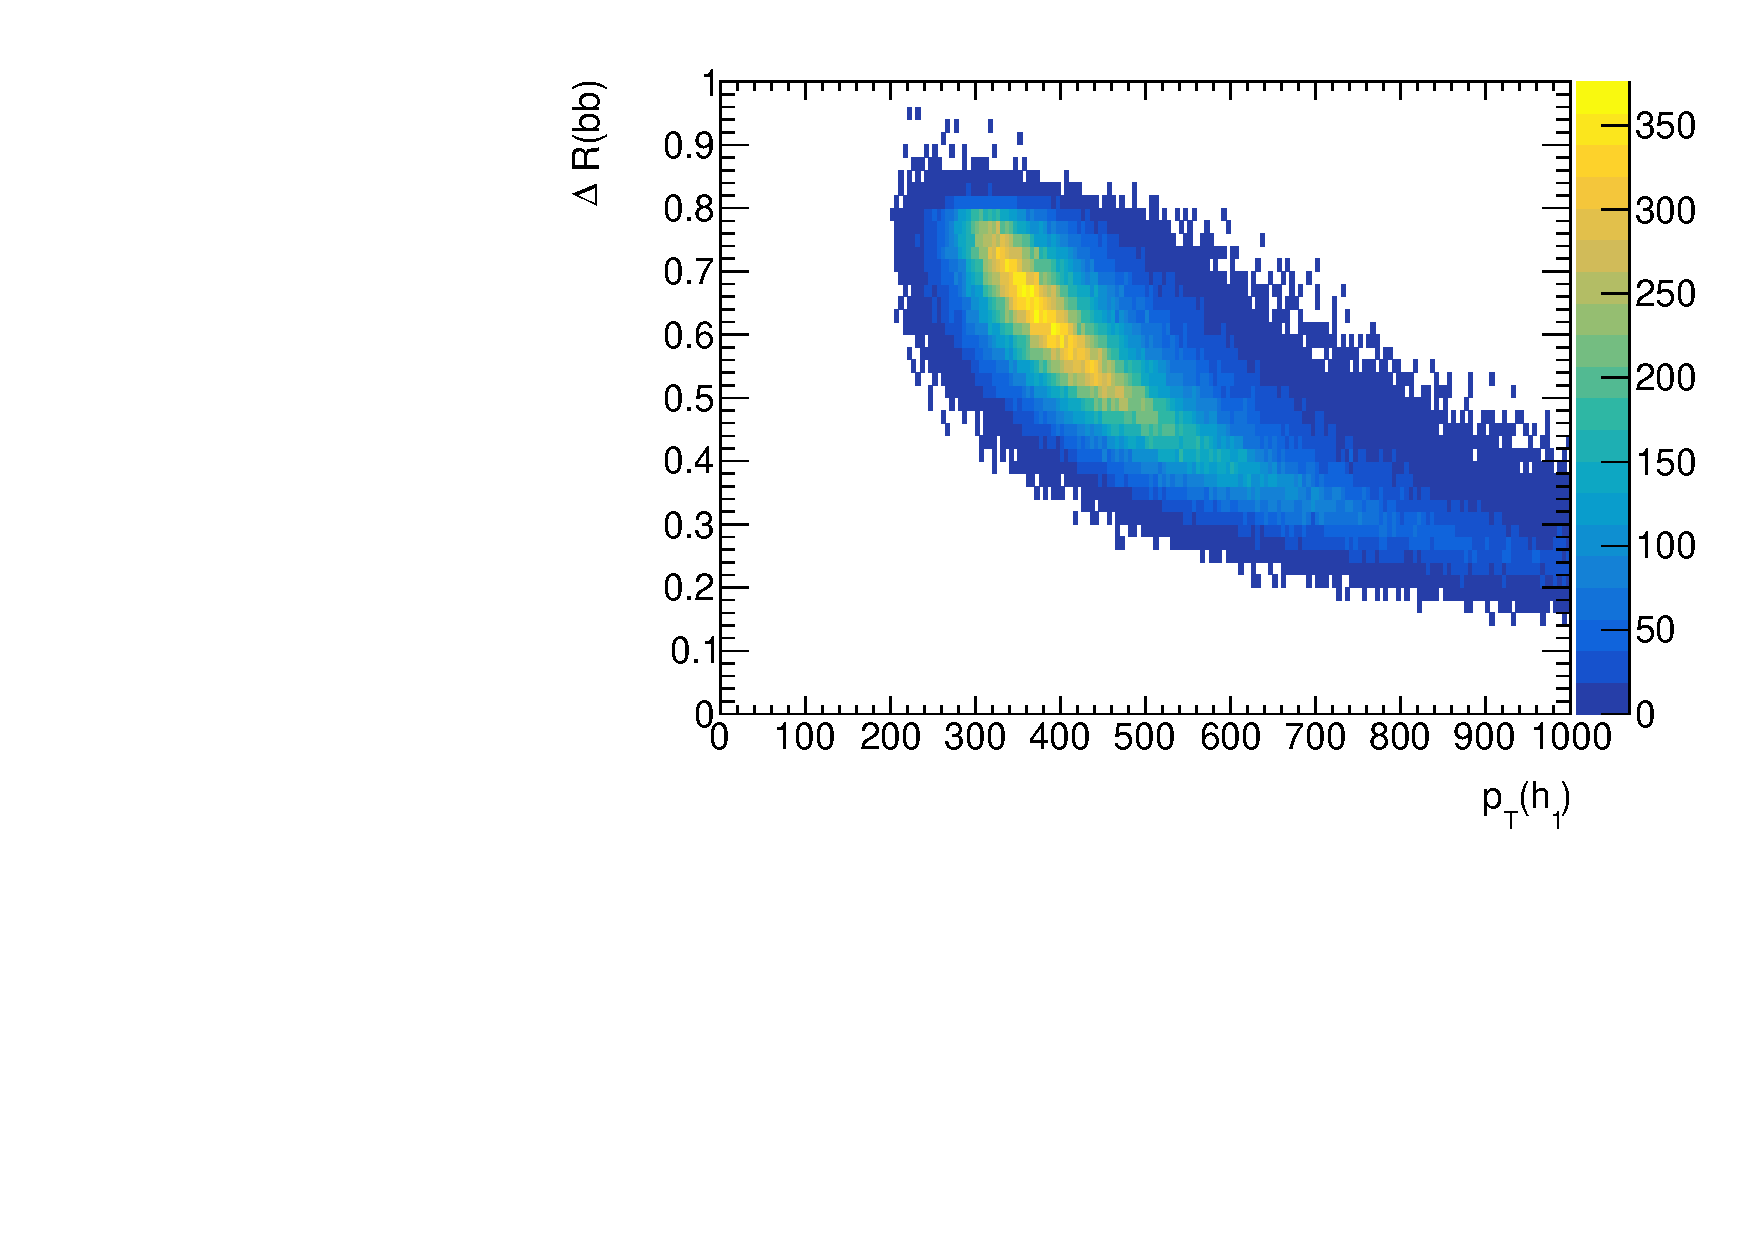
\includegraphics[width=0.7\linewidth]{./Figures/deltaR_bb_pt.pdf}
%	\label{fig:deltaR_bb_pt}
%	\caption{$\Delta R$ between the b quarks coming from the decay of the leading Higgs candidate, $h_1$. Plot obtained after the pre-selection cuts.}
%\end{figure}

%In the boosted regime, we expect at least two jets that are reconstructed using a large R parameter and that contain, each, the two b quarks that come from the decay of a Higgs boson. In the fully resolved regime, we expect at least four jets reconstructed with the standard R parameter of $0.4$, each corresponding to a b quark. Furthermore, an intermediate (or semi-resolved) category, in which one of the Higgs can be fully reconstructed using two small R jets and the other is reconstructed using a single large-R jet can also be explored. In all categories, we expect the presence of extra jets due to QCD activity. 

\subsection{Backgrounds}

The relevant backgrounds for this analysis are QCD (light?)multijet production, $t\overline{t}$ and $b\overline{b}b\overline{b}$. Although the $b\overline{b}b\overline{b}$ background is a particular case of a QCD multijet production process we consider it separately because it constitutes the irreducible background and therefore it will have a higher efficiency in the analysis. The cross sections for these processes are several orders of magnitude larger than the cross section for the signal, as Table \ref{table:samples_summary} shows. In addition, in the case of the $t\overline{t}$ background, the event topology is expected to be similar to the signal because it also consists in the production of a pair of particles with the same mass.

The assumption that QCD multijet production and $t\overline{t}$ two main backgrounds is corroborated by the ATLAS di-Higgs search performed in the same channel where these backgrounds are found to be the dominant ones and that all other sources of backgrounds, including processes involving Higgs bosons, are found to be negligible \cite{hh2bbbbATLAS}. In appendix \ref{chapter:bkgHiggs} we discuss and evaluate the importance of some backgrounds that include Higgs bosons to our analysis.

Figure \ref{fig:QCD} shows examples of LO Feynman diagrams that contribute to $b\overline{b}b\overline{b}$+j (left), three (middle) and four (right) light jets production. The $b\overline{b}b\overline{b}$ background is generated with an extra light jet at generator level. This jet boosts the four b quarks and has a minimum $p_T$ of $200$ GeV. This increases the probability of two b quarks being reconstructed as single large R jet therefore emulating the signal's final state signature. The QCD multijet background consists of two, three and four jet events (represented as jj+0/1/2 j), at generator level. The jets can originated from light and b quarks and from gluons. A jet matching procedure is implemented in Pythia in order to avoid double counting. Due to mis tagging probabilities light and c jets can be identified as b jets. Although these probabilities are relatively small when compared to the b-tagging efficiency (see section \ref{sec:btagging}) the cross section of multijet processes is very large such that this background becomes dominant.

CROSS SECTION FOR THESE PROCESSES.

As anticipated, the $p_T$ spectrum of the multijet background is a lot softer than for the signal and remaining backgrounds, as it is shown on both plots of figure \ref{fig:h1h2_pt}. In addition, for this background the $\tau_{21}$ variable takes values close to one, as it is shown in figure \ref{fig:hh_deltaEta_h1_tau21} on the right. This indicates that the jets are not consistent with two subjets. 

Figure \ref{fig:tt} shows examples of LO Feynman diagrams that contribute to $t\overline{t}$ production through $q\overline{q}$ (left) and $gg$ (middle and right) fusion. The $t\overline{t}$ background is simulated with additional zero, one or two jets (represented as $t\overline{t}$+0/1/2 j), at generator level. The extra jets can originated from light and b quarks and from gluons. A jet matching procedure is implemented in Pythia in order to avoid double counting. The top quark has a very short life time, predicted to be $5\times 10^{-25}$ s, such that it decays before it can hadronize. This sample is inclusive in the top quark decay modes. However, the most favoured decay of the top quark is $t\rightarrow Wb$ with a branching ratio close to $96\%$ \cite{PDG2016}. Therefore, $t\overline{t}$ events will, most of the times, result in the $WWbb$ final state. We do not specify any decay mode for the $W$ such that the sample is also inclusive in the $W$ decay modes. The $W$ decays to hadrons $(W^+\rightarrow q\overline{q})$ and leptons $(W^+\rightarrow l^+\nu)$ with BR$(W^+\rightarrow q\overline{q})\sim 68\%$ and BR$(W^+\rightarrow l^+\nu)\sim 10\%$. If one (or both) $W$ bosons decays to hadrons then there will be additional jets in the final state. These can be b jets or can be misidentified as such. If both $W$ bosons decay to leptons there will still be at least two b jets in the final state, coming from the $t\overline{t}$ decay.

CROSS SECTION.

It is interesting to note that in the softdrop mass plot for the leading Higgs candidate (figure \ref{fig:h1_eta_M} on the right) the $t\overline{t}$ background (green line) shows a small peak around $170$ GeV. In this region, all the decay products of the top quark are contained inside the $R=0.8$ jet.

%In addition, we also take into account the irreducible background, $b\overline{b}b\overline{b}$ because it is expected to be the background with the highest efficiency.

\begin{figure}
	\centering
	\feynmandiagram[small,layered layout,horizontal=i1 to a] {% Draw the top and bottom lines
		i1 [particle=\(\overline{q}\)]-- [anti fermion] a-- [boson, edge label'=\(g/h/Z/\gamma\)]  b,
		i2 [particle=\(q\)]-- [fermion] c-- [gluon, edge label=\(g\)] d,
		% Draw the two internal fermion lines
		{ [  same layer] a -- [anti fermion] c},
		%f1  -- [fermion] b -- [fermion] f2 ,
		%f3  -- [fermion] f2 -- [gluon] g1 ,
		%f4  -- [fermion] g1 -- [fermion] f5 ,
		%	a -- [opacity=0.2] c,
		%g1 -- [anti fermion] b,
		b -- [anti fermion] f2 [particle=\(\overline{b}\)],
		b -- [fermion] f3 ,
		f3 -- [fermion] f4 [particle=\(b\)],
		f3 -- [boson, edge label'=\(g/h/Z/\gamma\)] g1,
		g1 -- [anti fermion] f5 [particle=\(\overline{b}\)],
		g1 -- [fermion] f6 [particle=\(b\)],
	};\qquad
	\feynmandiagram[small,layered layout,horizontal=a to b] {% Draw the top and bottom lines
		i1 [particle=\(\overline{q}\)]-- [anti fermion] a-- [anti fermion]  b,
		i2 [particle=\(q\)]-- [fermion] c-- [fermion] d [particle=\(q\)],
		% Draw the two internal fermion lines
		{ [  same layer] a -- [gluon] c},
		%f1  -- [fermion] b -- [fermion] f2 ,
		%f3  -- [fermion] f2 -- [gluon] g1 ,
		%f4  -- [fermion] g1 -- [fermion] f5 ,
		%	a -- [opacity=0.2] c,
		%g1 -- [anti fermion] b,
		b -- [anti fermion] f2 [particle=\(\overline{q}\)],
		b -- [gluon] f3 [particle=\(g\)],
	};\qquad
	\feynmandiagram
	[horizontal=a to b] {i1 [particle=\(q\)] -- [fermion] a -- [fermion] i2 [particle=\(\overline{q}\)],
		a -- [gluon] b,
		g1 -- [gluon] b -- [gluon] g2,
		f1 [particle=\(\overline{q}\)] -- [fermion] g1 -- [fermion] f2 [particle=\(q\)],
		f3 [particle=\(\overline{q}\)] -- [fermion] g2 -- [fermion] f4 [particle=\(q\)],
		g1 -- [opacity=0] g2,
		f2 -- [opacity=0] f4,
	};
	%		\feynmandiagram[small,layered layout,horizontal=i1 to a] {% Draw the top and bottom lines
	%			i1 [particle=\(\overline{q}\)]-- [anti fermion] a-- [boson, edge label'=\(h/Z/\gamma\)]  b,
	%			i2 [particle=\(q\)]-- [fermion] c-- [gluon, edge label=\(g\)] d,
	%			% Draw the two internal fermion lines
	%			{ [  same layer] a -- [anti fermion] c},
	%			%f1  -- [fermion] b -- [fermion] f2 ,
	%			%f3  -- [fermion] f2 -- [gluon] g1 ,
	%			%f4  -- [fermion] g1 -- [fermion] f5 ,
	%			%	a -- [opacity=0.2] c,
	%			%g1 -- [anti fermion] b,
	%			b -- [anti fermion] f2 [particle=\(\overline{b}\)],
	%			b -- [fermion] f3 ,
	%			f3 -- [fermion] f4 [particle=\(b\)],
	%			f3 -- [boson, edge label'=\(h/Z/\gamma\)] g1,
	%			g1 -- [anti fermion] f5 [particle=\(\overline{b}\)],
	%			g1 -- [fermion] f6 [particle=\(b\)],
	%		};
	\label{fig:QCD}
	\caption{Example of diagrams that contribute to the QCD multijet background: five final state jets, four of which are b-jets (left), three final state jets (middle) and four final state jets (right). Here, $q$ stands for a light quark/jet.}
\end{figure}

\begin{figure}
\centering
\feynmandiagram
[horizontal=a to b] {i1 [particle=\(q\)] -- [fermion] a -- [fermion] i2 [particle=\(\overline{q}\)],a -- [gluon,edge label=\(g\)] b, f1 [particle=\(t\)] -- [fermion] b -- [fermion] f2 [particle=\(\overline{t}\)],
};\qquad
\feynmandiagram
[horizontal=a to b] {i1 [particle=\(g\)] -- [gluon] a -- [gluon] i2 [particle=\(g\)],a -- [gluon,edge label=\(g\)] b, f1 [particle=\(t\)] -- [fermion] b -- [fermion] f2 [particle=\(\overline{t}\)],
}; \qquad
\feynmandiagram[layered layout,horizontal=a to b] {% Draw the top and bottom lines
	i1 [particle=\(g\)]-- [gluon] a-- [anti fermion]  b [particle=\(\overline{t}\)] -- ,i2 [particle=\(g\)]-- [gluon] c-- [fermion] d [particle=\(t\)] -- ,
	% Draw the two internal fermion lines
	{ [  same layer] a -- [fermion] c},
};
\label{fig:tt}
\caption{Dominant diagrams of $pp\rightarrow t\overline{t}$ at LO.}
\end{figure}


%\begin{figure}[h]
%	\centering
%	\feynmandiagram [horizontal=b to c] {
%		a -- [gluon] b [blob],c -- [scalar] b-- [gluon] d,
%		c -- [scalar] e,
%		c -- [scalar] f,
%		e -- [fermion] g,
%		e -- [anti fermion] h,
%		f -- [fermion] i,
%		f -- [anti fermion] j,
%	};
%	\caption{Final state}
%\end{figure}

%\begin{figure}[h]
%	\centering
%	\feynmandiagram [horizontal=d to h] {
%		a [particle=\(g\)] -- [gluon] b [blob],
%		c [particle=\(g\)] -- [gluon] b -- [gluon],
%		d -- [scalar, edge label'=\(h\)] b -- [scalar],
%		e -- [scalar, edge label'=\(h\)] b -- [scalar],
%		d -- [fermion, edge label=\(b\)] g ,
%		d -- [anti fermion, edge label=\(\overline{b}\)] h ,
%		e -- [fermion, edge label'=\(b\)] i,
%		e -- [anti fermion, edge label'=\(\overline{b}\)] j ,
%		d -- [opacity=0] e,
%		%h -- [opacity=0] i,
%		g -- [opacity=0] h,
%		i -- [opacity=0] j,
%		h -- [opacity=0] i,
%	};
%	\caption{Final state}
%\end{figure}




%\begin{table}
%	\centering
%	\begin{tabular}{lp{30mm}p{10mm}p{30mm}p{30mm}}
%		\toprule 
%		Pythia & hh (h$\rightarrow b\overline{b}$) & 4b+j & jj+0/1/2 j & tt+0/1/2 j \\
%		\midrule
%		Relevant settings & 25:onMode=off \newline 25:onIfAny= 5 -5&  & \textbf{Jet matching:} \newline merge=on \newline scheme=1 \newline setMad=off \newline coneRadius=1.0 \newline etaJetMax=10 \newline nJetMax=4 \newline qCut=30 & \textbf{Jet matching:} \newline merge=on \newline scheme=1 \newline setMad=off \newline coneRadius=1.0 \newline etaJetMax=10 \newline nJetMax=2 \newline qCut=60\\
%		\rowcolor{black!7} Description & Turn on the $h\rightarrow b\overline{b}$ decay for the undecayed Higgs. &  &  \multicolumn{2}{l}{Set parameters for jet matching procedure. } \\
%		\bottomrule
%	\end{tabular}
%	\caption{oi}
%	\label{table:DelphesHCAL}
%\end{table}

\begin{figure}
	\centering
	\begin{minipage}{.5\textwidth}
		\centering
		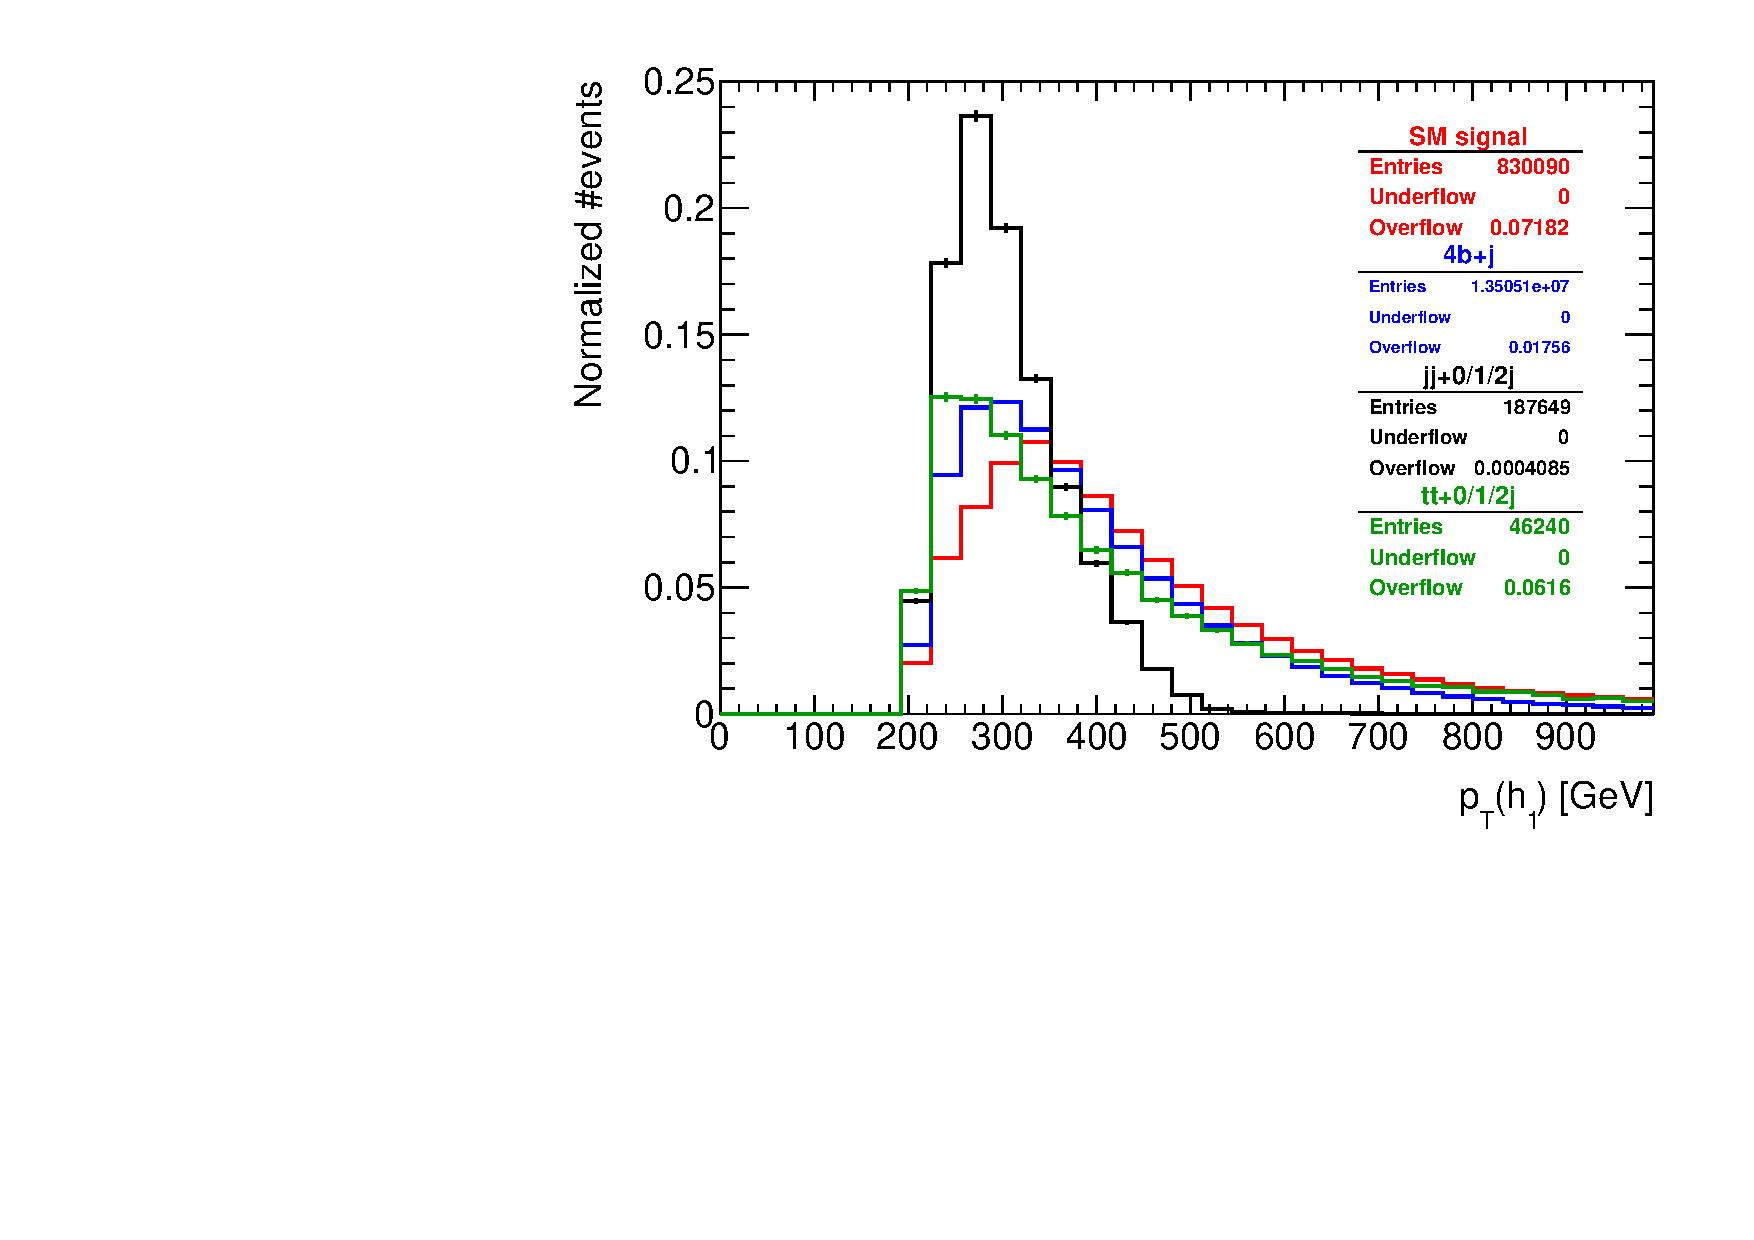
\includegraphics[trim={.65cm 0 0 0},clip,width=\linewidth]{./Figures/hist_h1_pt.pdf}
		%\caption{oi}
		%\label{fig:h1_pt}
	\end{minipage}%
	\begin{minipage}{.5\textwidth}
		\centering
		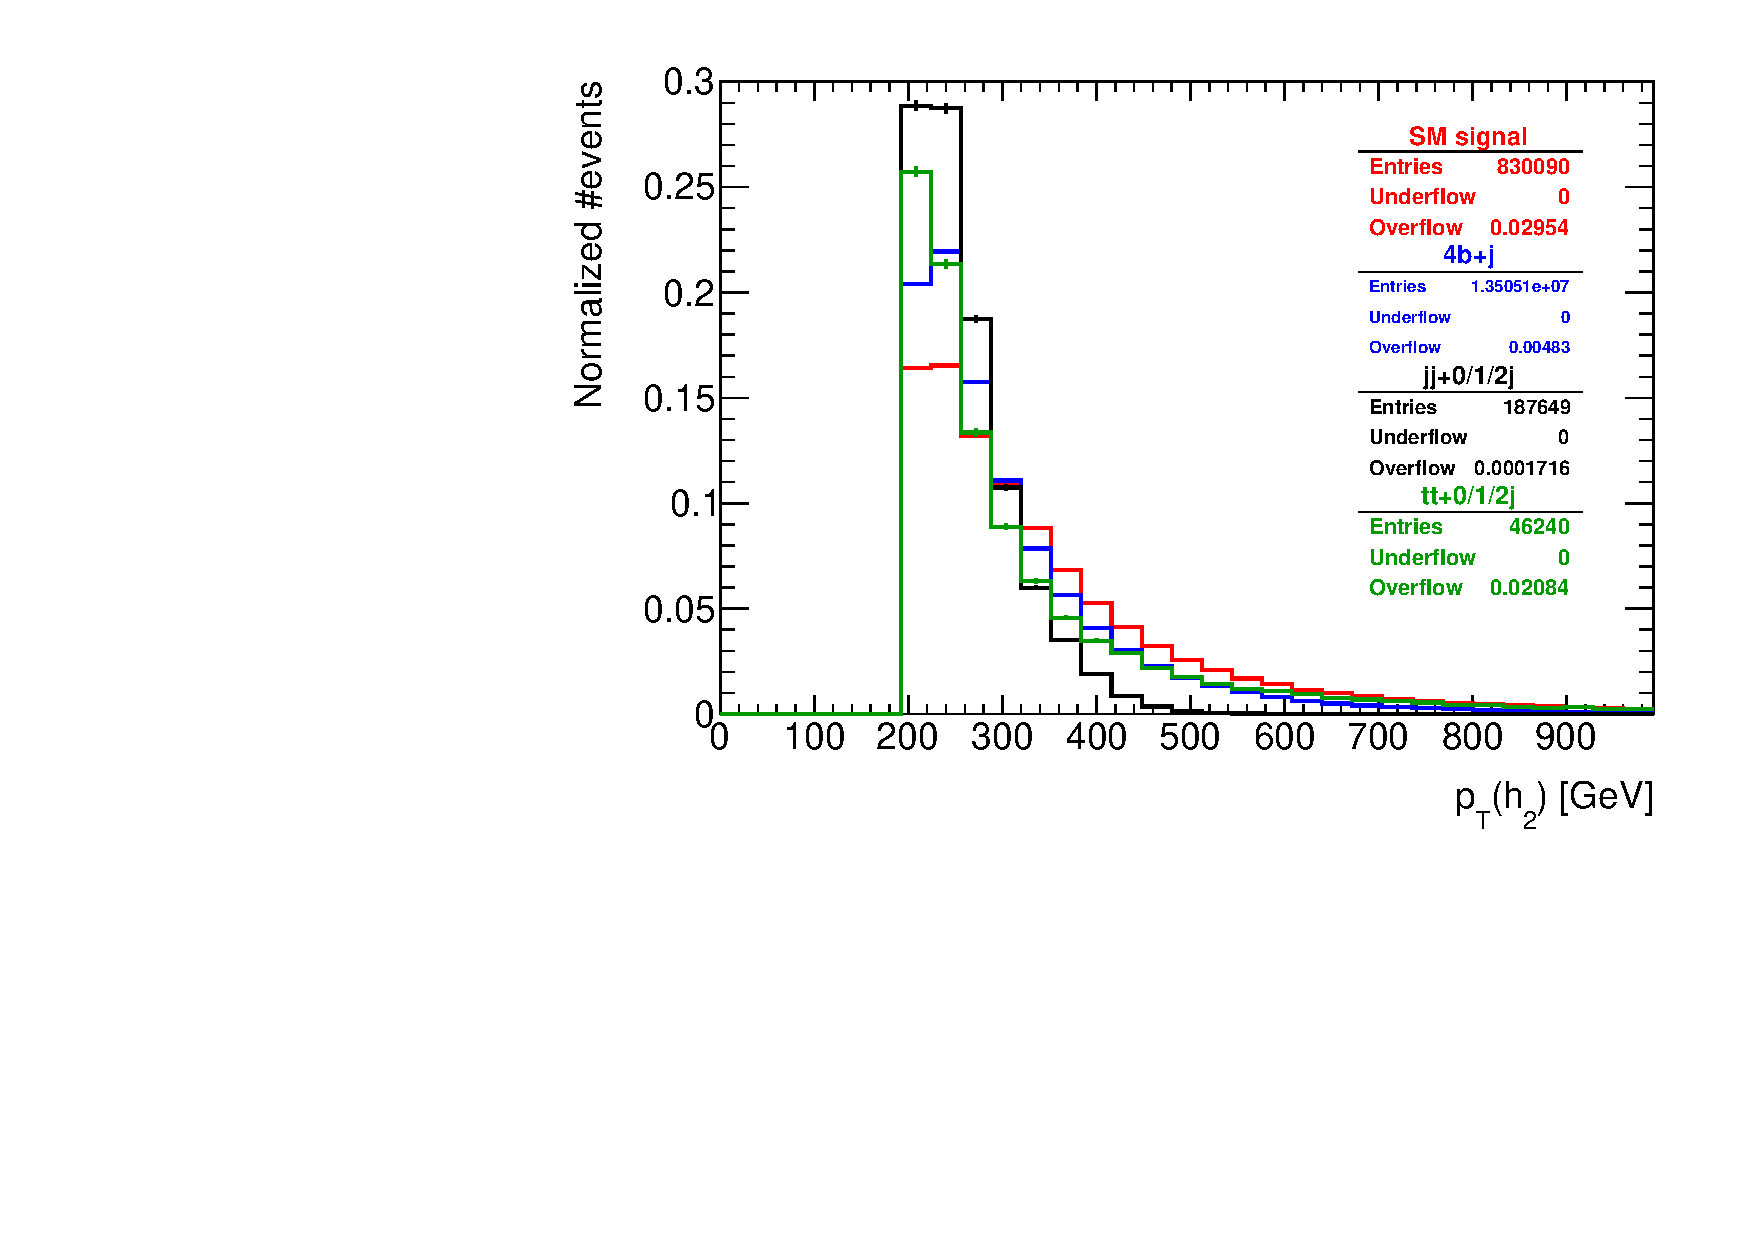
\includegraphics[trim={0 0 .65cm 0},clip,width=\linewidth]{./Figures/hist_h2_pt.pdf}
		%\caption{oi}
		%\label{fig:h2_pt}
	\end{minipage}
	\label{fig:h1h2_pt}
	\caption{$p_T$ distributions for the leading (left) and sub leading (right) Higgs candidates. The signal is the SM $hh\rightarrow b\overline{b}$ process. The histograms are normalized to unit area.}
\end{figure}

\begin{figure}
	\centering
	\begin{minipage}{.5\textwidth}
		\centering
		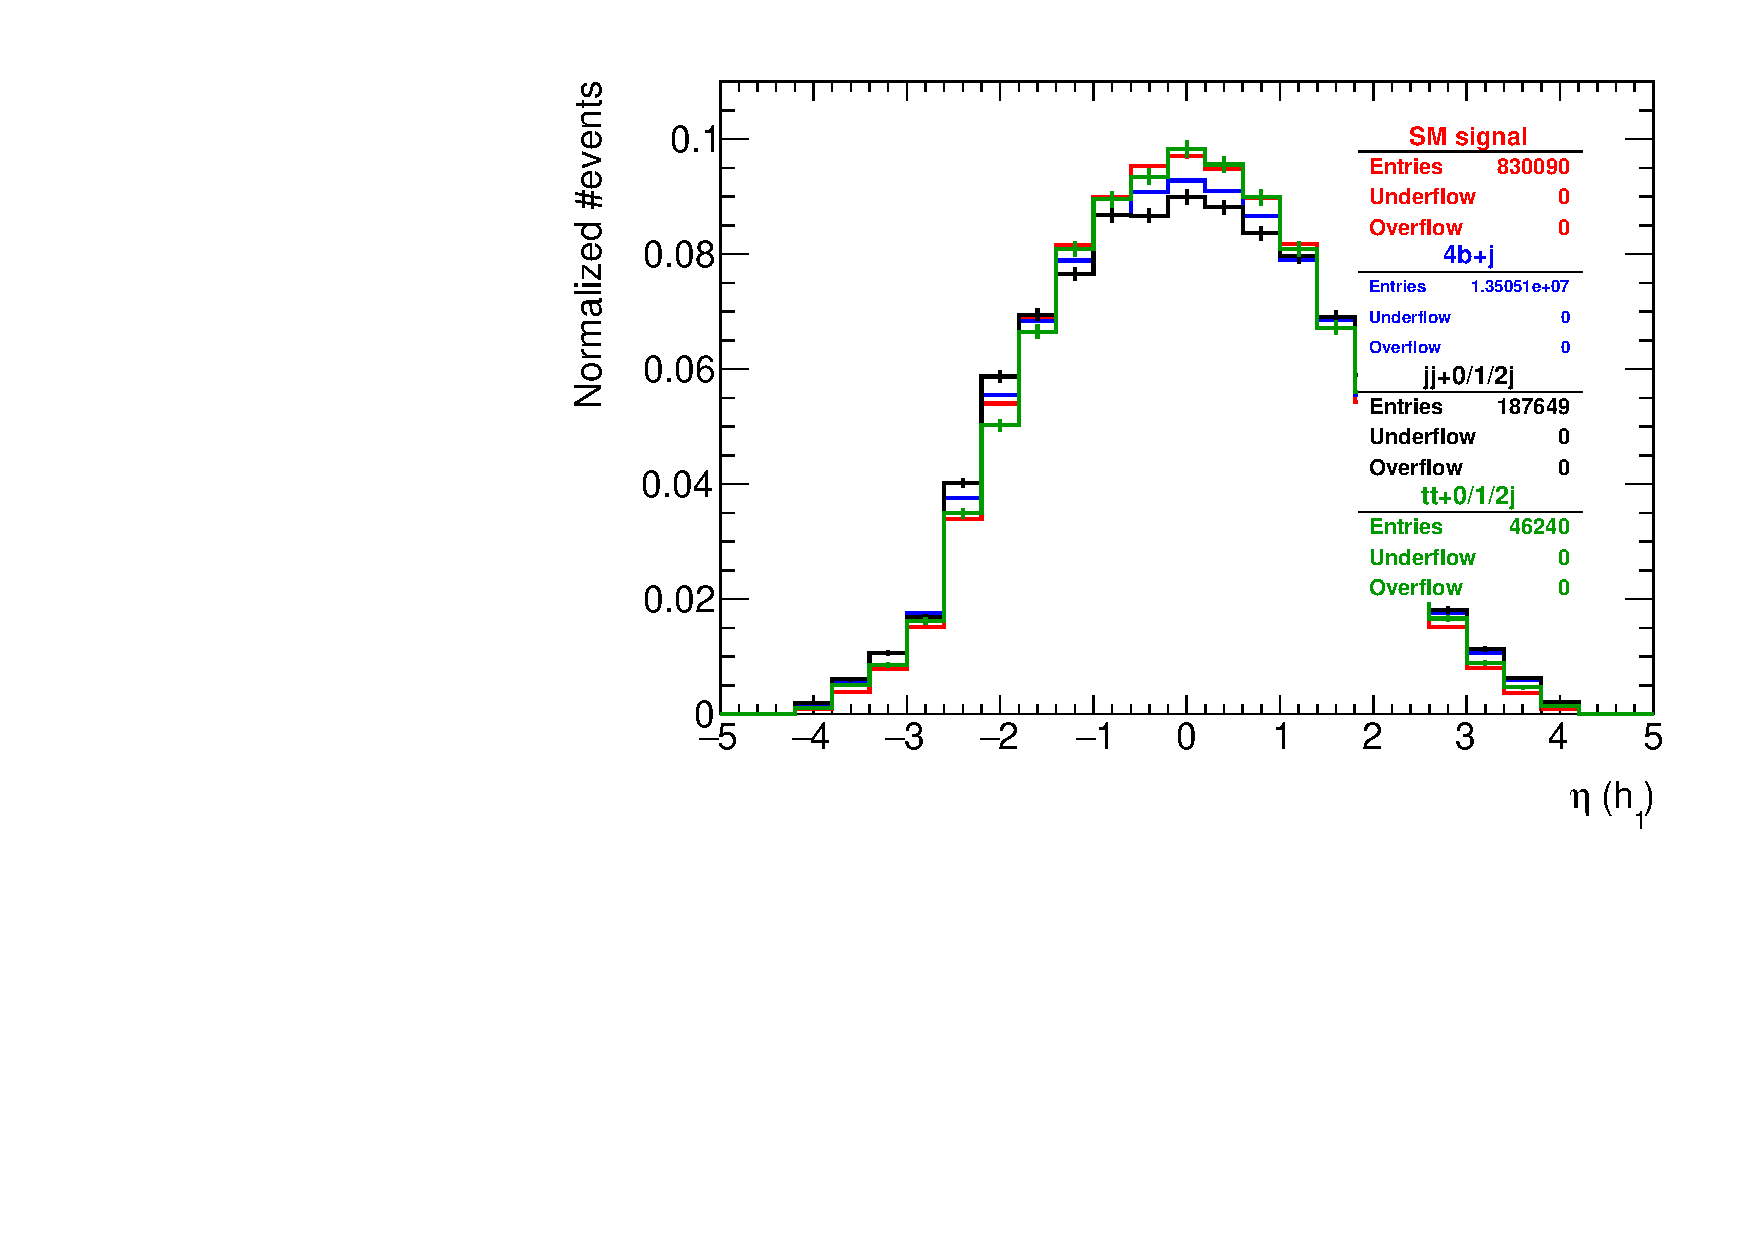
\includegraphics[trim={.65cm 0 0 0},clip,width=\linewidth]{./Figures/hist_h1_eta.pdf}
		%\caption{oi}
		%\label{fig:h1_pt}
	\end{minipage}%
	\begin{minipage}{.5\textwidth}
		\centering
		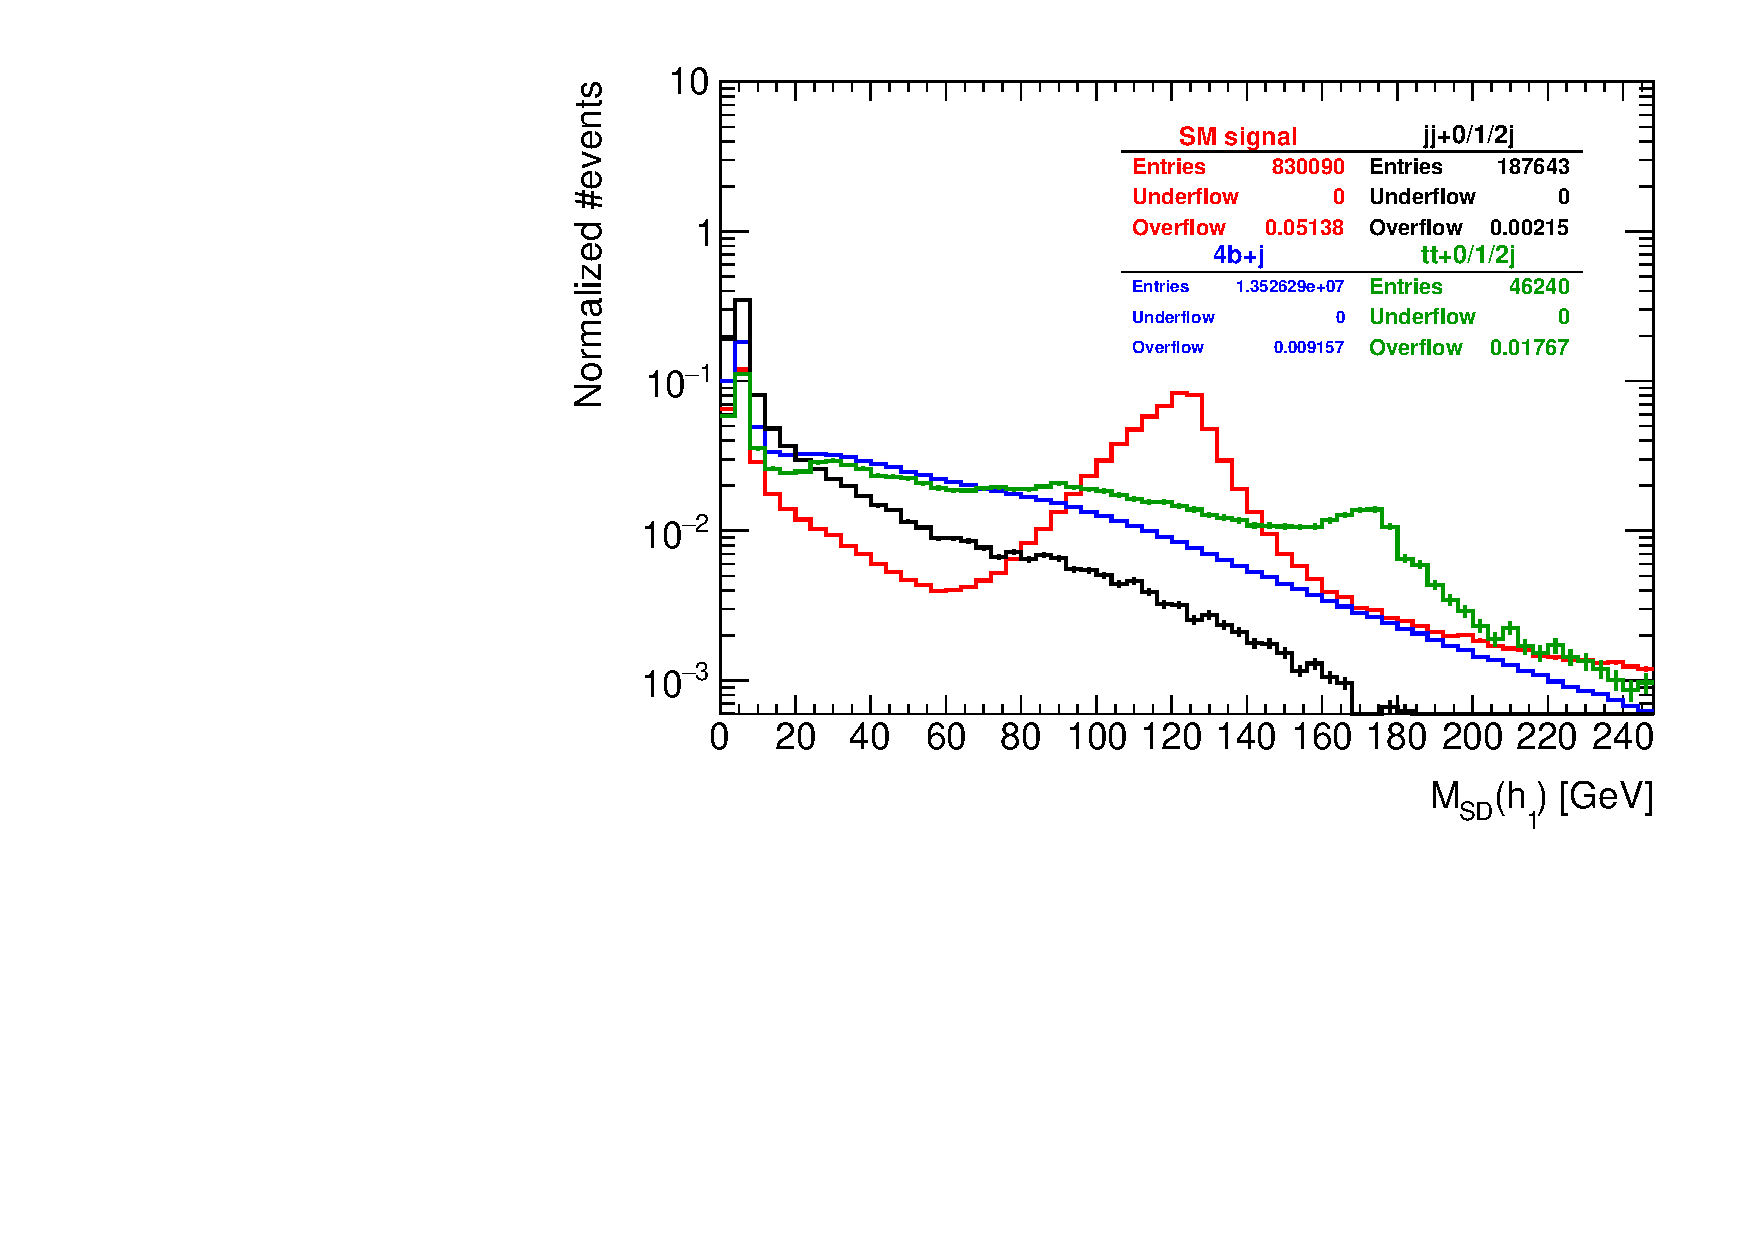
\includegraphics[trim={0 0 .65cm 0},clip,width=\linewidth]{./Figures/hist_h1_softdrop_M.pdf}
		%\caption{oi}
		%\label{fig:h2_pt}
	\end{minipage}
	\label{fig:h1_eta_M}
	\caption{$\eta$ distribution for the leading Higgs candidate (left) and softdrop mass distribution for the leading Higgs candidate (right). The signal is the SM $hh\rightarrow b\overline{b}$ process. The histograms are normalized to unit area.}
\end{figure}	

\begin{figure}
	\centering
	\begin{minipage}{.5\textwidth}
		\centering
		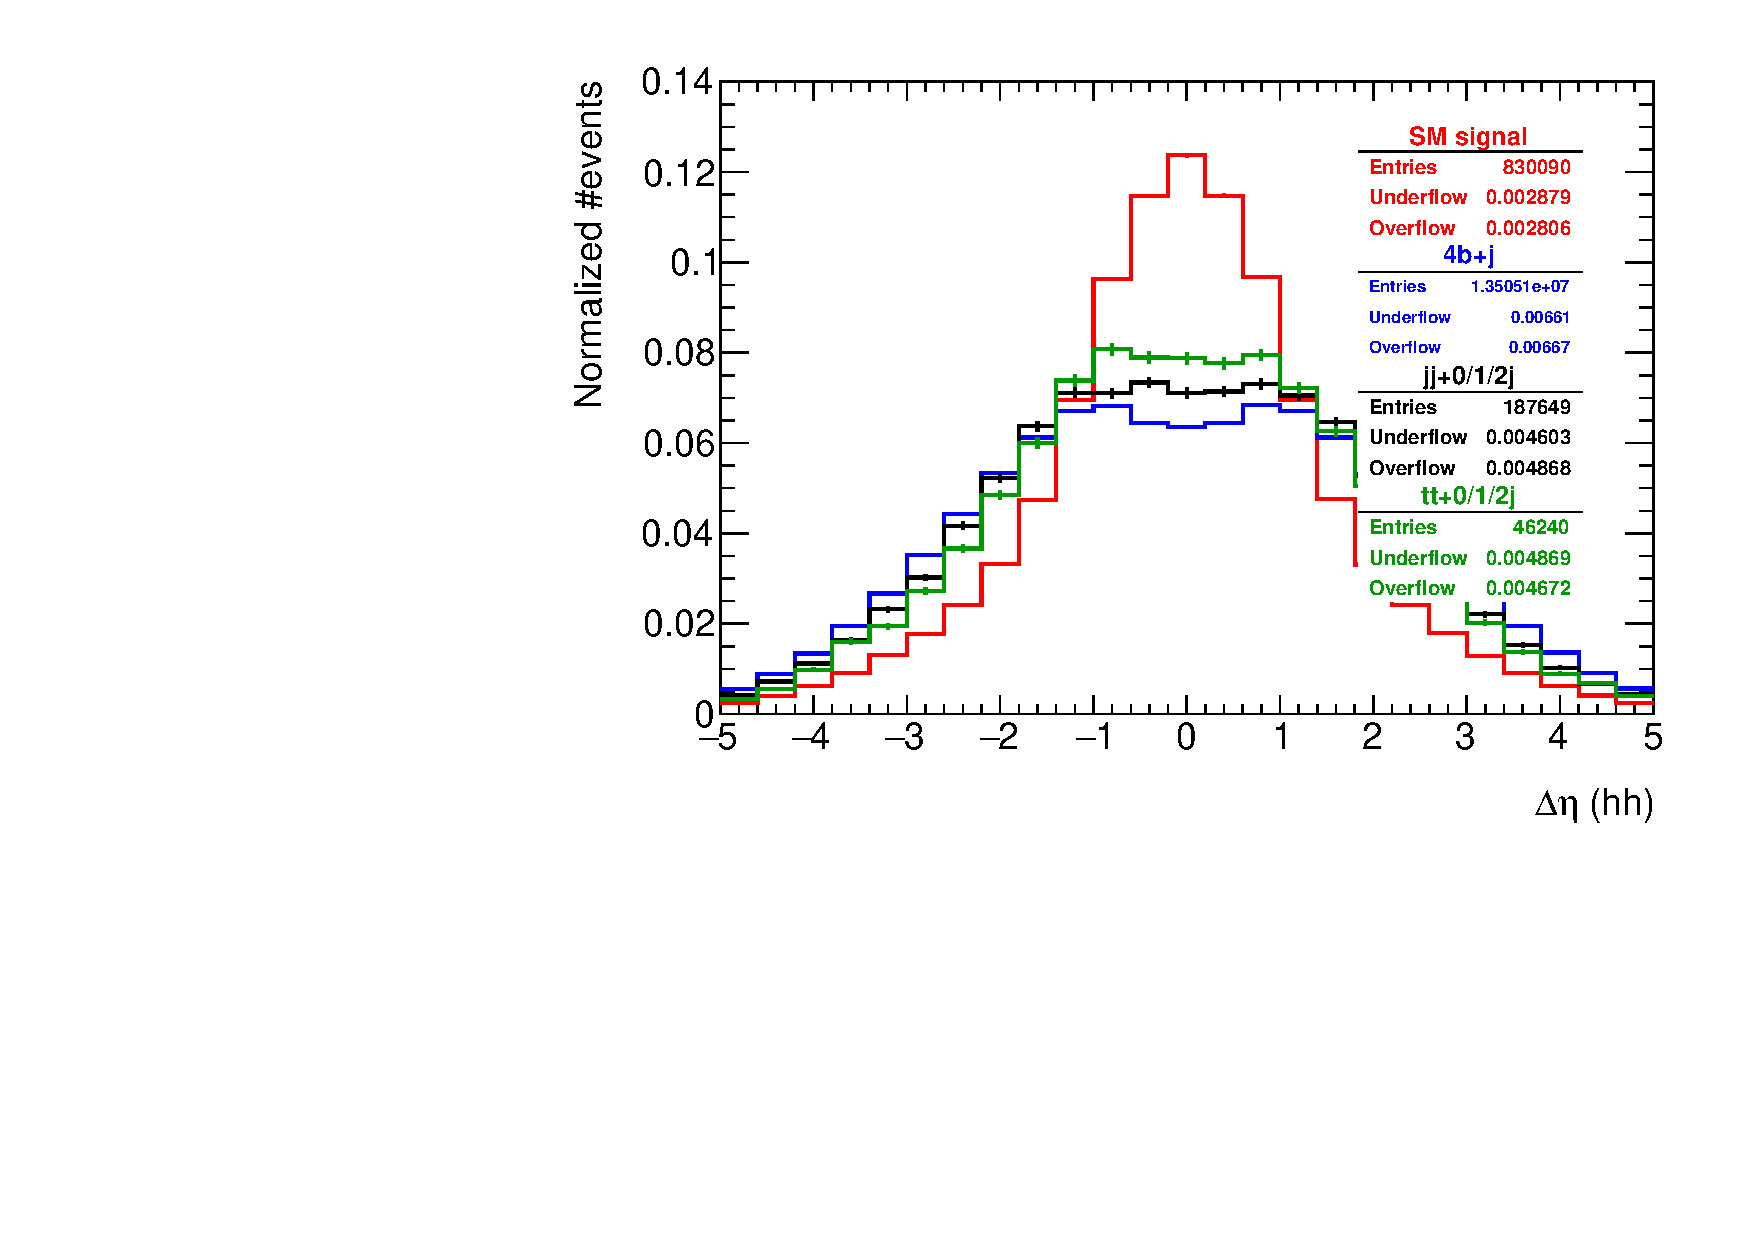
\includegraphics[trim={.65cm 0 0 0},clip,width=\linewidth]{./Figures/hist_hh_deltaEta.pdf}
		%\caption{oi}
		%\label{fig:h1_pt}
	\end{minipage}%
	\begin{minipage}{.5\textwidth}
		\centering
		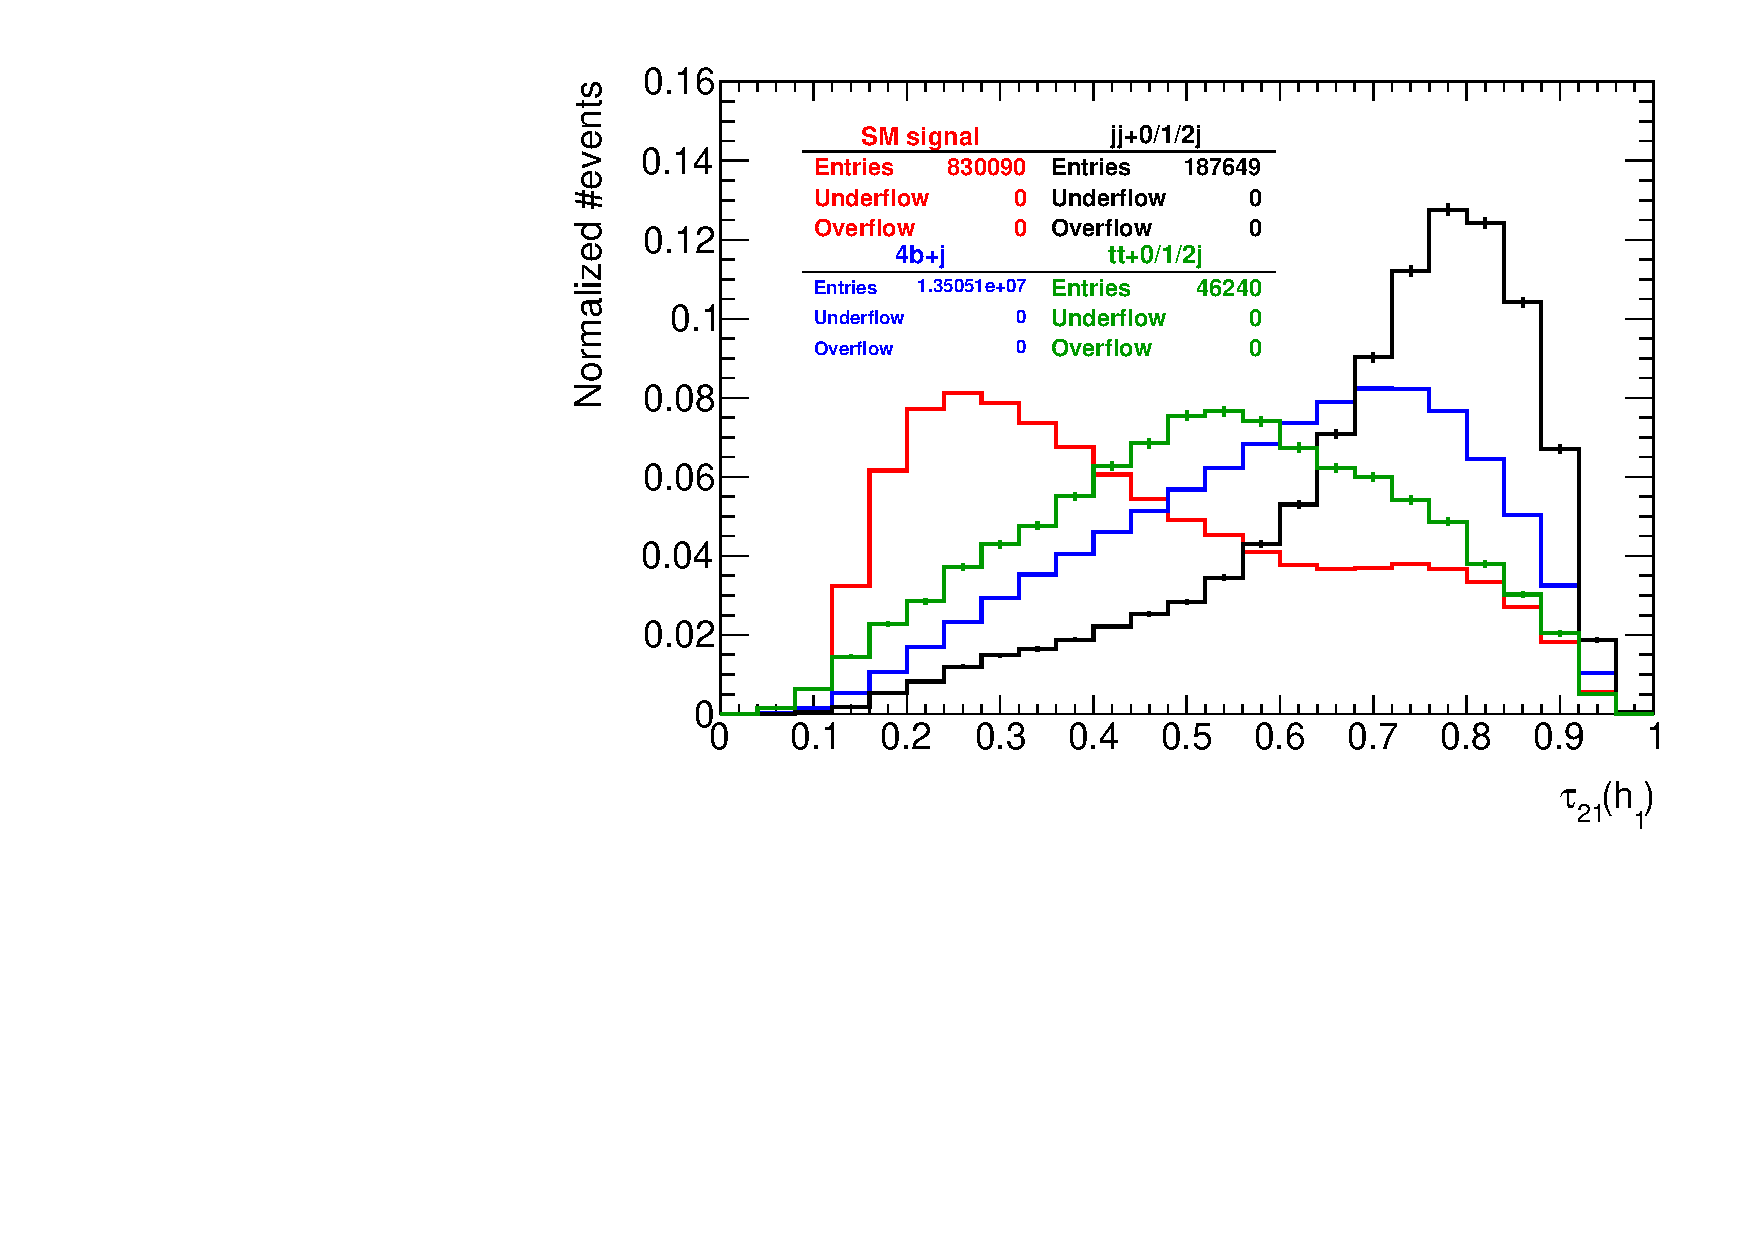
\includegraphics[trim={0 0 .65cm 0},clip,width=\linewidth]{./Figures/hist_h1_tau21.pdf}
			%\caption{oi}
			%\label{fig:h2_pt}
		\end{minipage}
		\label{fig:hh_deltaEta_h1_tau21}
		\caption{oi}
\end{figure}
	

\section{Analysis strategy}
\label{section:regions}

-------------------------------------------------------------------\\
%In this analysis we explore three regions: boosted, intermediate and resolved. The details about each region, namely the event topology and selection cuts, are discuss in the following sections (\ref{section:boosted}, \ref{section:intermediate} and \ref{section:resolved}). The regions are orthogonal, i.e, independent. For each event we check if it falls in the boosted category. If it does not we check if it falls in the intermediate category and if it does not we check if it falls in the resolved category. This way, an event falling in the boosted category cannot fall in the intermediate or resolved categories and the same applies for all categories. 
%
%The advantage of performing an analysis in orthogonal regions is that we can then combine the results obtained in each one. For example, we can quadratically add the significances in order to obtained an overall significance. This would not be possible if there were any overlap between the regions. In addition, we have access to increased statistics because we are exploring three different signal topologies. Nonetheless, the selection criteria for each category, as well as the variables to explore, are different and need to be optimized independently.

- Event topology: two boosted jets each corresponding to a Higgs \\
- Physics objects: partile flow anti-kT R=0.8 jets (discussion about jet radius in appendix) \\
- Selection criteria\\
- Substructure variables \\
- Optimization (efficiency plots, correlations, MVA...)\\
-------------------------------------------------------------------

%\begin{figure}
%	\centering
%	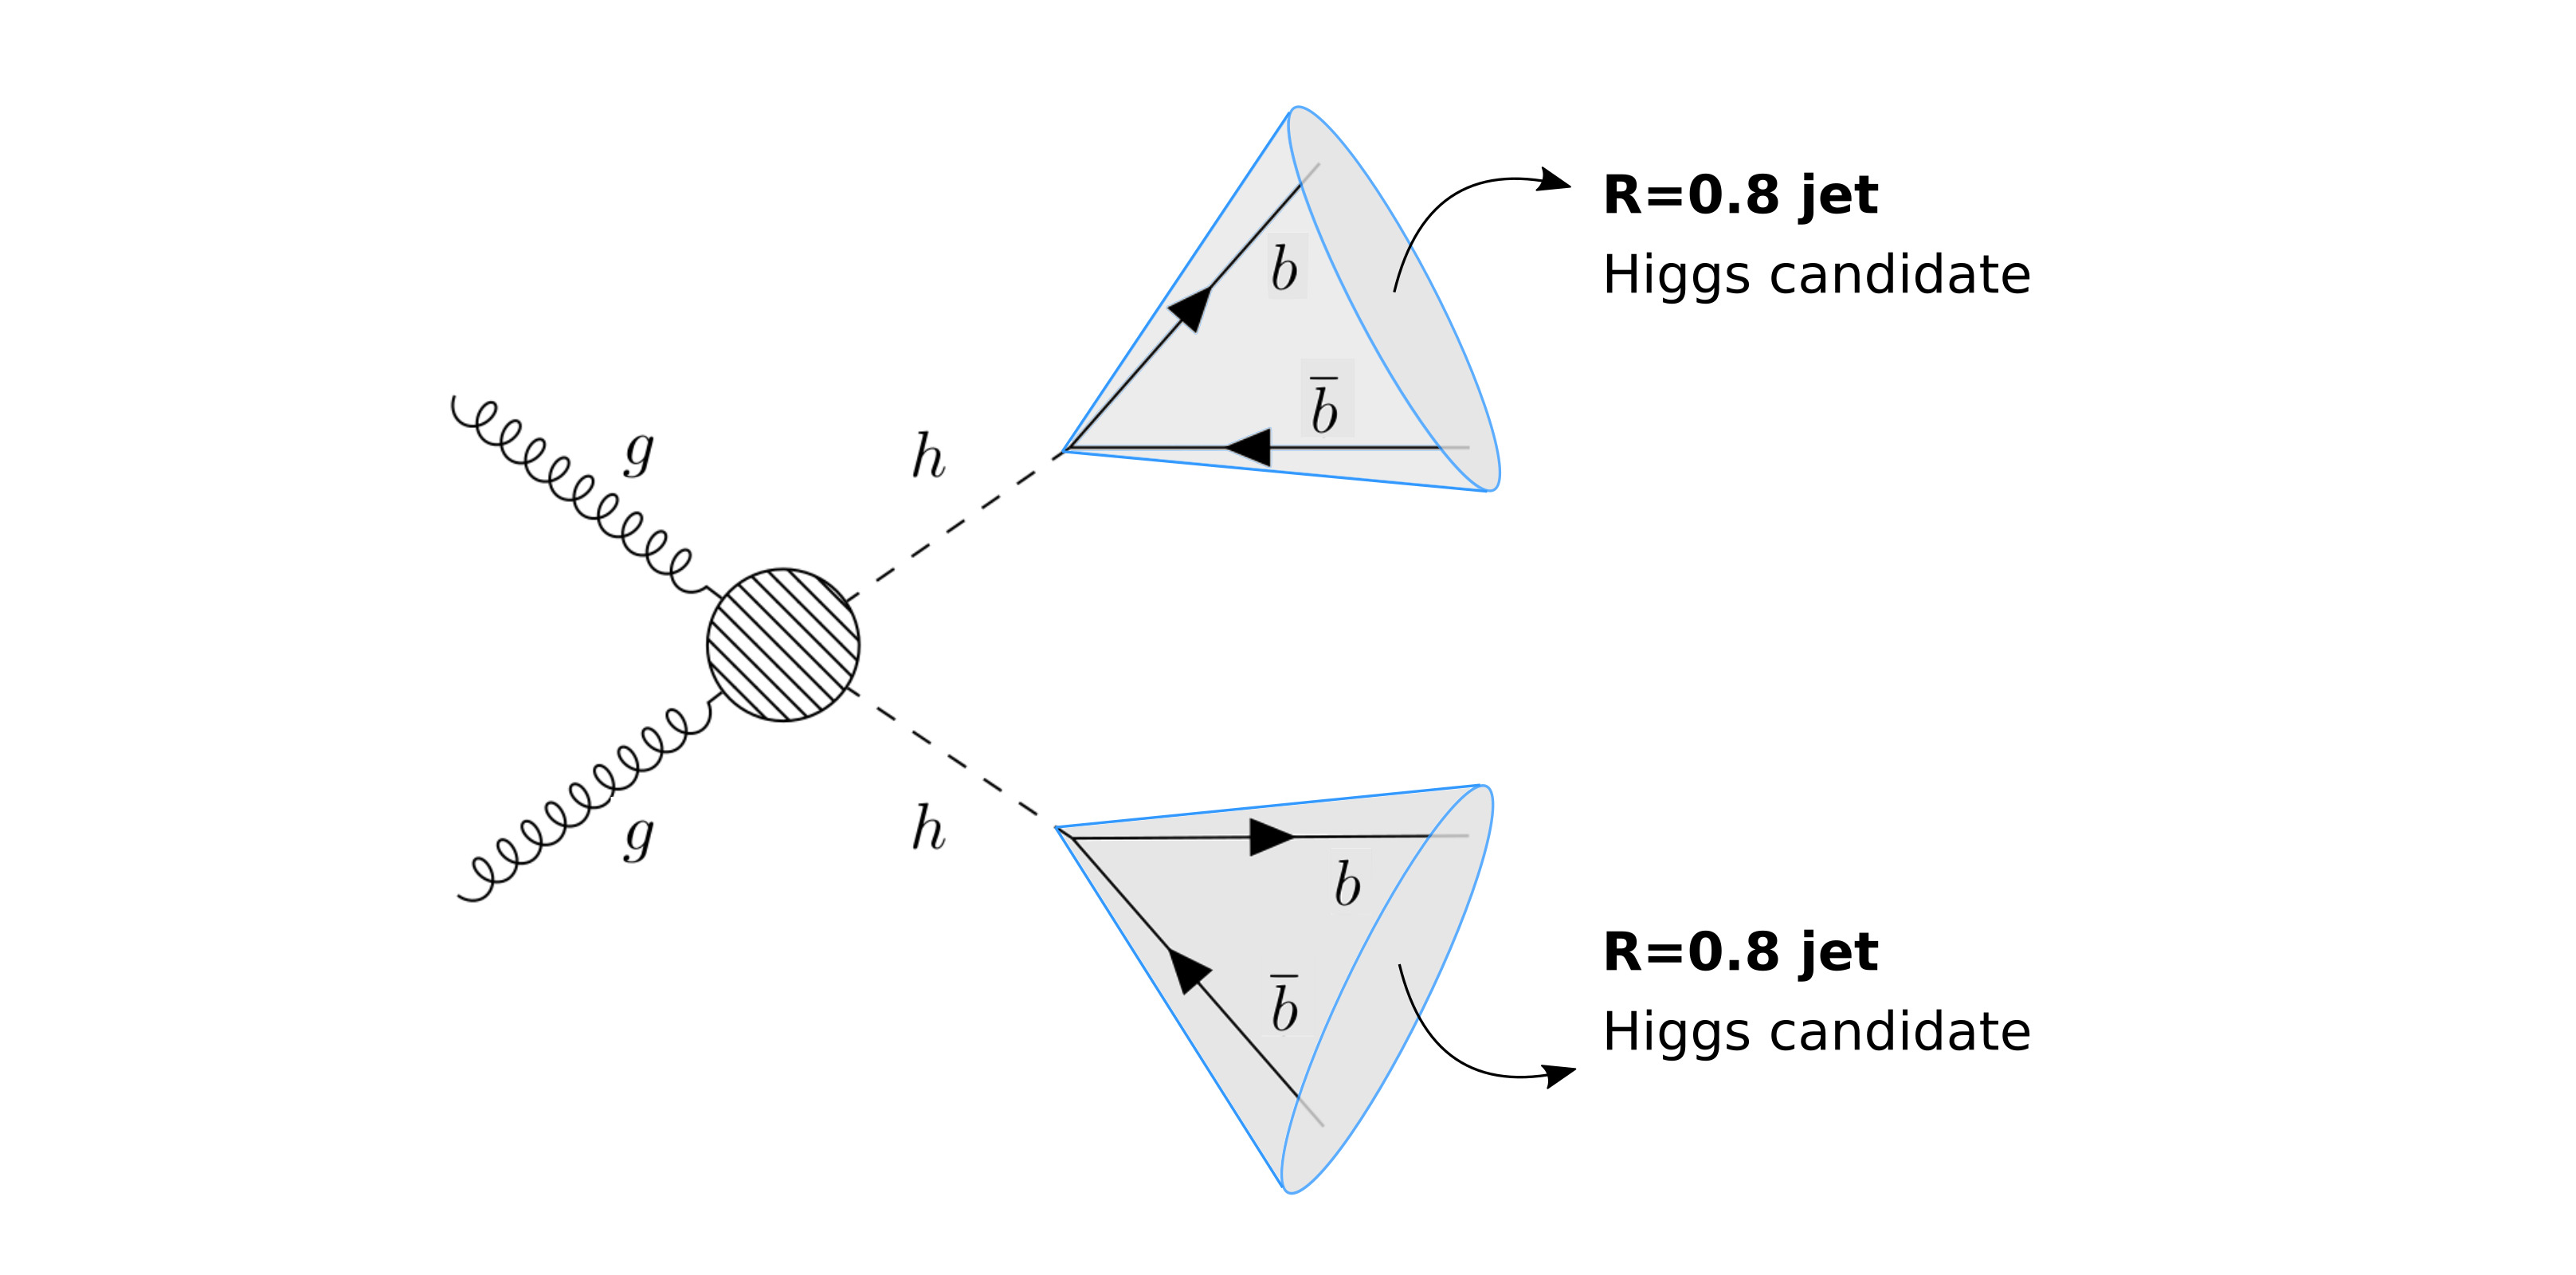
\includegraphics[width=\textwidth]{./Figures/boosted1.png}
%	%\hfill
%	%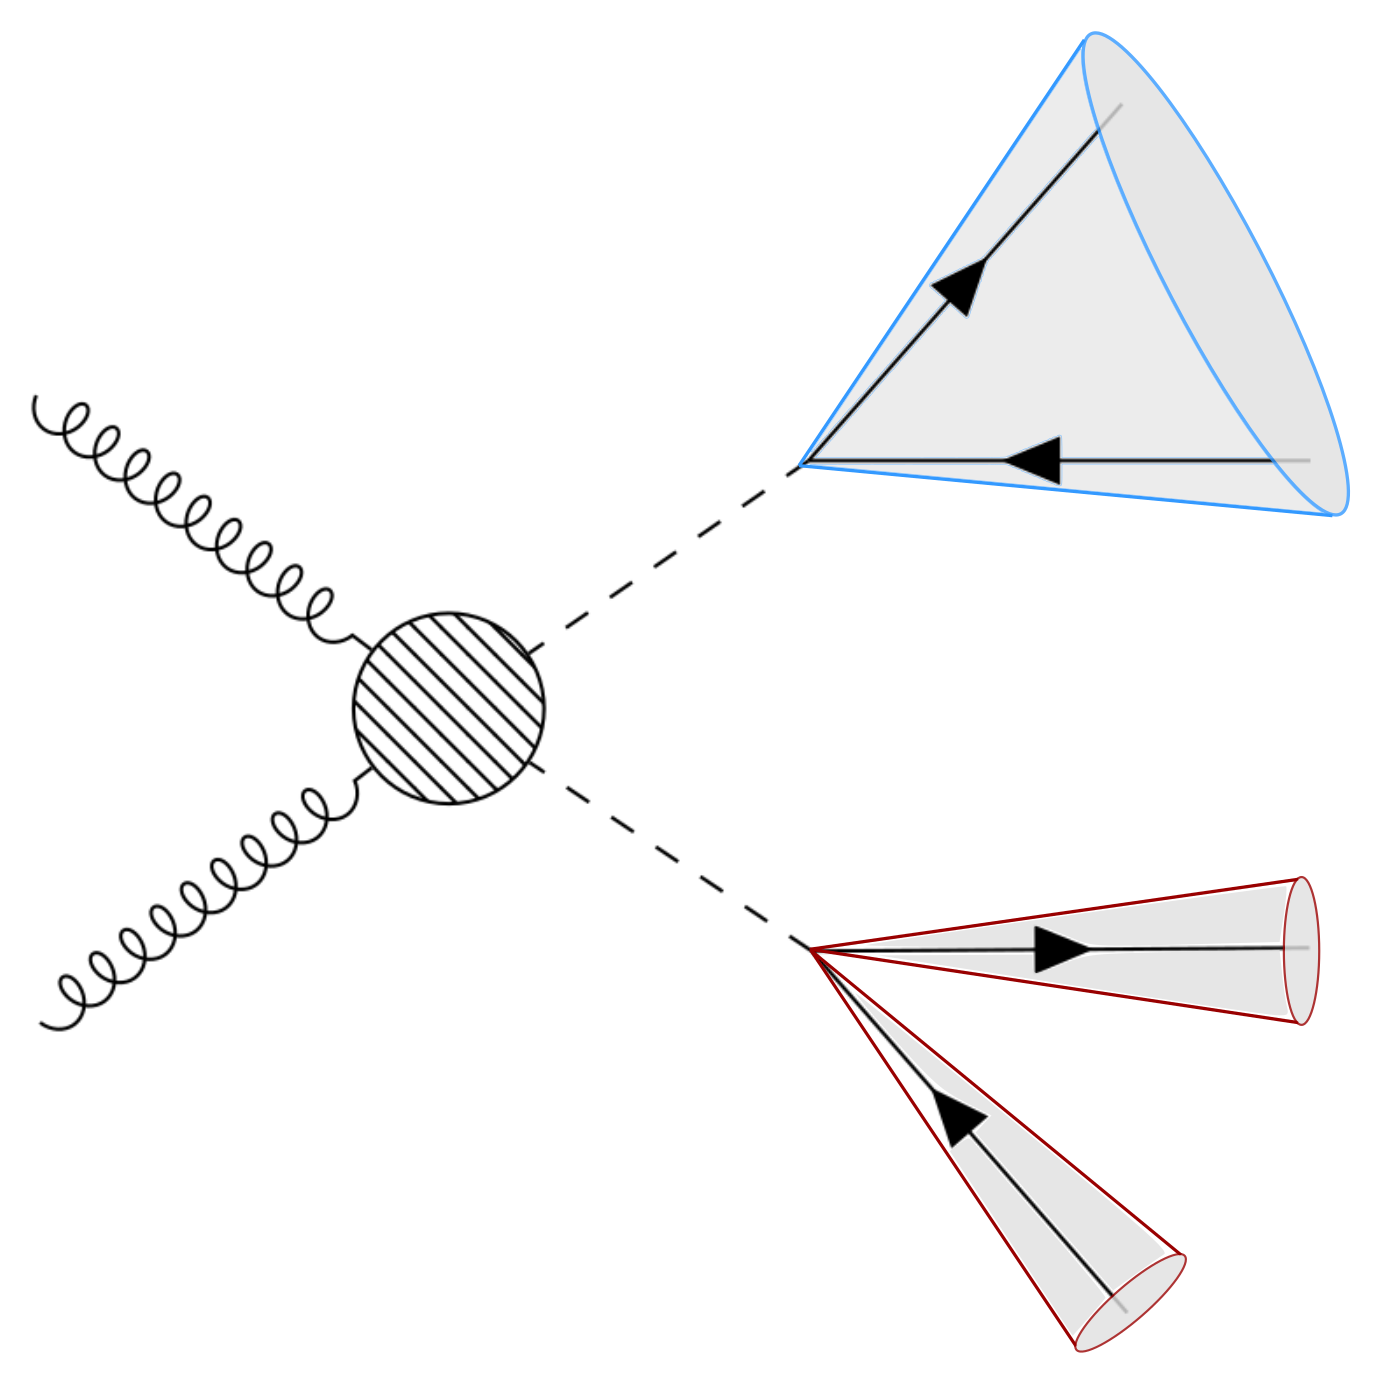
\includegraphics[width=.45\textwidth]{./Figures/inter.png}
%	\caption{Event topology targeted by the boosted analysis region. The blob represents the interaction between the gluons and the Higg bosons that is represented by the Feynman diagrams shown in figure \ref{fig:higgs_pair}.}
%	\label{fig:final_state}
%\end{figure} 

%In this analysis is focused on the bosoted regime. It targets events in which the Higgs bosons have a high Lorentz boost which leads to the collimation of the pairs of b quarks resulting from their decay. As a result, the b quarks cannot be reconstructed in four separated jets. Therefore, two pairs of b quarks are reconstructed using two jets with a larger R parameter. Each jet is expected to contain the b quarks coming from one of the Higgs bosons and works as a proxy for the properties of that Higgs boson.

This analysis targets events in which at least two large R jets are reconstructed. The jet with the highest momentum is assumed to correspond to the leading Higgs candidate and the jet with the second highest momentum to the sub leading one. Both the leading and sub leading jets must be b-tagged in order for the event to be accepted.

The events are reconstructed using particle flow (or eflow) or pure calormeter jets (we explored both approaches) with $R=0.8$, clustered with the anti-$k_T$ algorithm. We perform the b-tagging of jets using truth level information as it is described in the following section. Jets with a large R parameter cannot be b-tagged using Delphes default algorithm because the tagging of large R jets is an ambiguous task that can be performed in several different ways. Therefore, we implemented our own b-tagging algorithm/strategy that is described in section \ref{sec:btagging}. 

\subsection{Implementation of b-tagging}
\label{sec:btagging}

\begin{wrapfigure}{R}{0.5\textwidth}
	\centering
	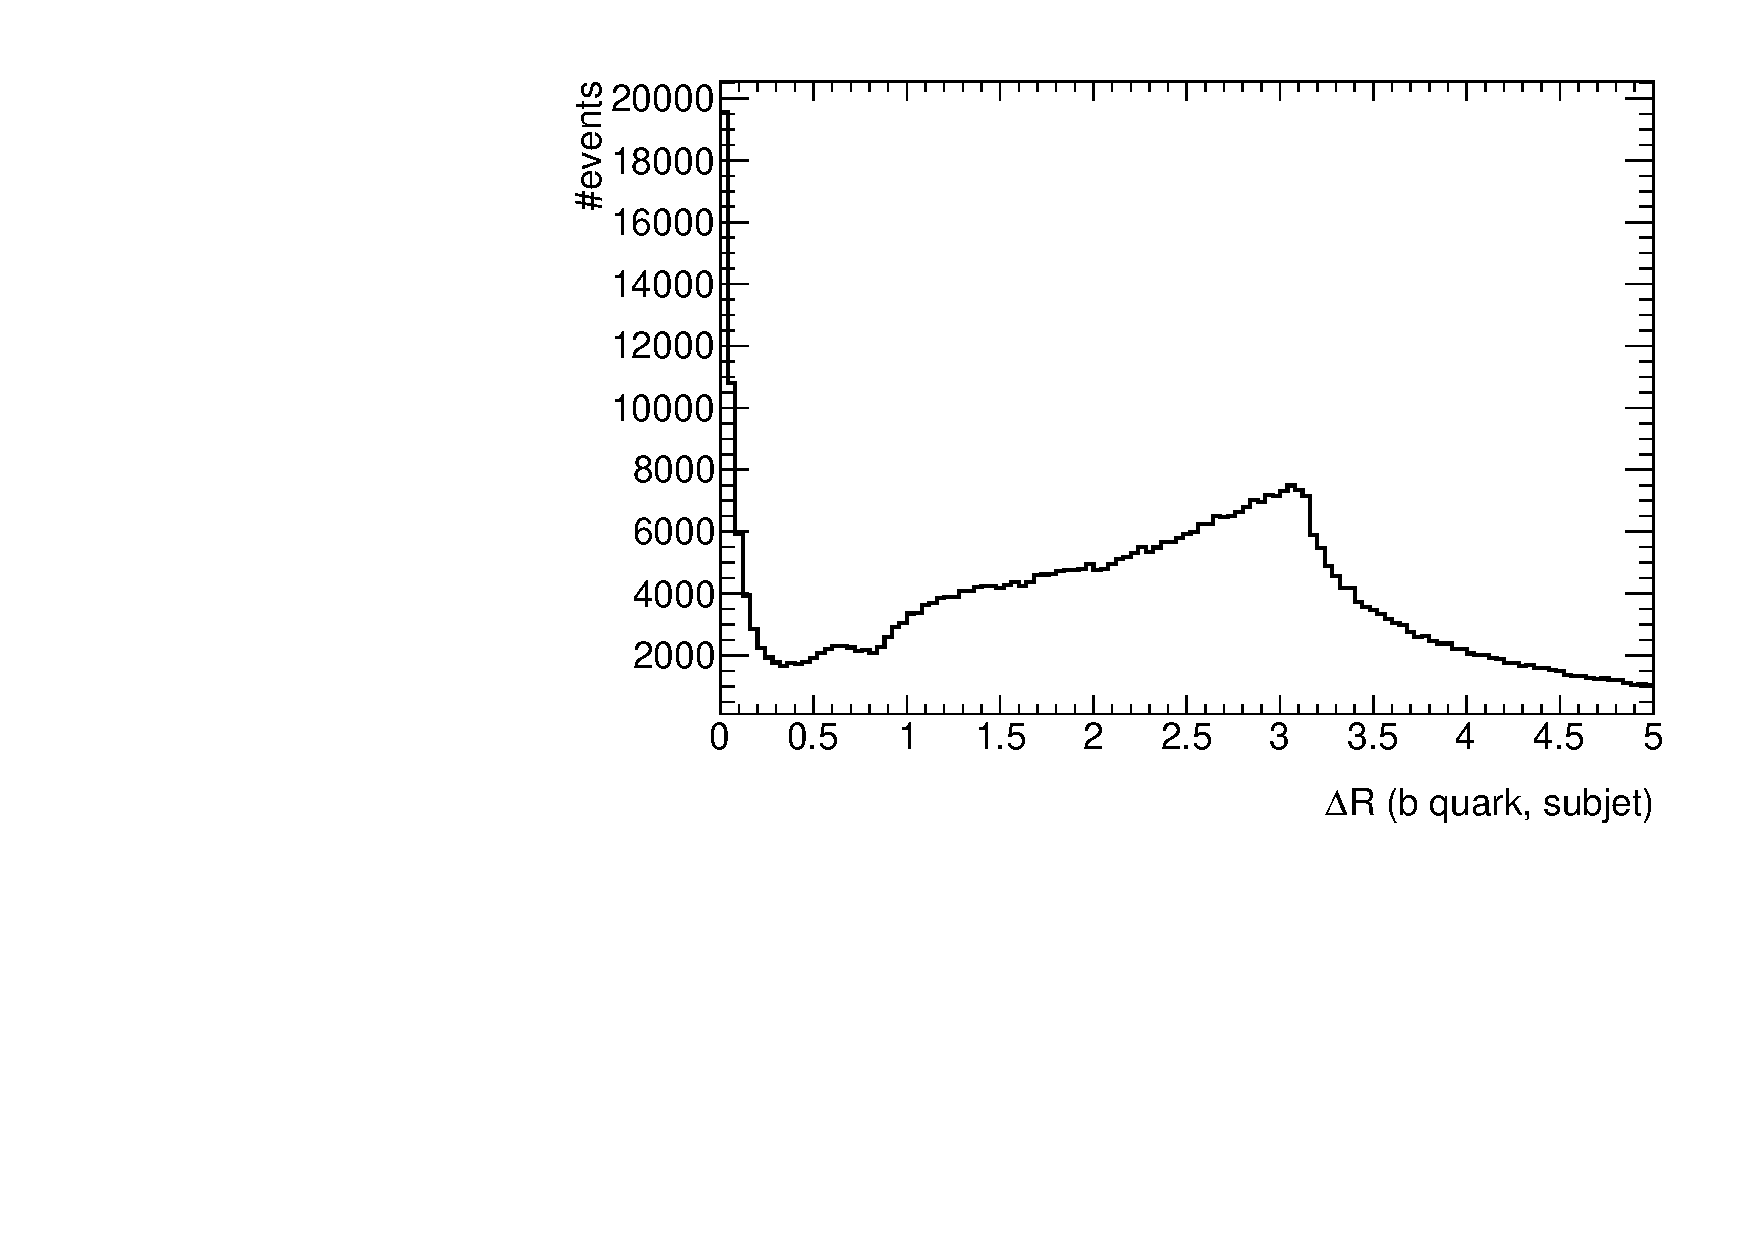
\includegraphics[width=0.5\textwidth]{./Figures/deltaR_bsubjet}
	\caption{Minimun $\Delta R$ between b quarks and subjets of the $R=0.8$ jets.} 
	\label{fig:deltaR_bsubjet}
\end{wrapfigure}

For each jet, the two hardest subjets are found using the mass drop procedure. It might happen that there are not two subjets because the algorithm's criteria are not met. In that case, the jet is rejected. We compute the $\Delta R$ distance between all b and c quarks in the event with Pythia 8 status equal to $23$ and with $p_T>10$ GeV and each subjet, $\Delta R(\text{subjet,parton})$. According to the Pyhtia manual, particles with status $23$ result directly from the hardest subprocess. We consider that a subjet is matched to a given quark if $\Delta R(\text{subjet,parton})<0.3$, as indicated by the plot in Figure \ref{fig:deltaR_bsubjet}. In this plot there is a peak for $\Delta R<0.3$ that corresponds to the  If the subjet is matched to at least a b quark, we b-tag the subjet with a given probability. If the subjet is not matched to any b quark but it is matched to at least one c quark we apply a c mistag rate. If the subjet is not matched to any b or c quark we apply a light mistag rate. The b-tag probability and mistag rates were obtained from the Delphes FCC-hh card. They depend on the momentum of the jet and on its $\eta$ coordinate. They are summarized in Table \ref{table:btag}. Note that a jet cannot be b-tagged if $|\eta|>4$ or if its momentum is smaller than $10$ GeV or larger than $15000$ GeV. 



\begin{table}
	\centering
	\begin{tabular}{llll}
		\toprule 
		\backslashbox{$\eta$}{$p_T$} & $10<p_T<500$ & $500<p_T<15000$ &  \\
		\midrule
		$|\eta|<2.5$ & $0.85;\textcolor{blue}{0.05};\textcolor{red}{0.01} $ & $(0.85;\textcolor{blue}{0.05};\textcolor{red}{0.01})\times\left(1-p_T/15000\right)$ &   \\
		\rowcolor{black!7} $2.5<|\eta|<4.0$ & $0.64;\textcolor{blue}{0.03};\textcolor{red}{0.0075}$ & $(0.64;\textcolor{blue}{0.03};\textcolor{red}{0.0075})\times\left(1-p_T/15000\right)$ &  \\
		\bottomrule
	\end{tabular}
	\caption{b-Tagging (black), c (blue) and light (red) mistag probabilities as a function of $\eta$ and $p_T$ of the (sub)jet. The momentum dependent factor, $\left(1-p_T/15000\right)$, is common to the three probabilities.}
	\label{table:btag}
\end{table}

%\subsection{Event pre-selection}
%
%TO INCLUDE: \\
%- discussion on trigger requirements: important in real analysis\\
%- show and discuss some distributions: invariant mass (h, hh), momentum, tau21, delta eta (hh), more substructure variables (may be all that we considered relevant)\\
%- compare with other articles/analysis ? \\
%
%--------------------------------------------------------------------------------------------------
%
%We require at least two b-tagged $R=0.8$ jets (which corresponds to at least four b-tagged subjets, at least two in each $R=0.8$ jet). In addition, the leading and sub leading jets must have $p_T\geq200$ GeV in order for the event to be accepted. Due to the b-tagging efficiency formulas, there is a natural cutoff at $|\eta|=4$ so we do not place any additional cut in $\eta$. From now on, these cuts are referred to as pre-selection cuts. 

\subsection{Baseline analysis}

The analysis described in this section and on the ones that follow were developed using the sample simulated with the default FCC-hh detector implementation. The analysis was then applied to the samples generated using the different detector configurations. This allows for a straightforward comparison between the significances.

As a first step, we implemented a baseline analysis based on rectangular cuts on kinematic and substructure variables. Firstly, we apply cuts on the transverse momentums of the leading and sub leading Higgs candidates, $p_T(h_1)$ and $p_T(h_2)$,and of the Higgs pair, $p_T(hh)$:
\begin{equation}
	p_T(h_1)>400 ~\text{GeV}, \quad p_T(h_2)>350 ~\text{GeV}, \quad p_T(hh)>100 ~\text{GeV}.
\end{equation}
These cuts follow from both distributions shown in figure \ref{fig:pt_stack} and guarantee that we are choosing events for which the Higgs candidates are sufficiently boosted. In addition, a high threshold for the $p_T$ of the jets suppresses $t\overline{t}$ events because the decay products of the top quark are reconstructed in a single jet. In a real analysis, these cuts would also be dictated by the trigger threshold. 

From figure \ref{fig:sub_stack}, on the left, we then apply a cut on the $\tau_{21}$ of the leading Higgs candidate to select jets that are more compatible with a "2-prong" structure:
\begin{equation}
	\tau_{21}(h_1)<0.55.
\end{equation}
The cut on this variable works as an Higgs tagging method. Therefore we apply the same cut on the $\tau_{21}$ of the sub leading Higgs candidate although that does not necessarily follow from the distribution on the right of figure \ref{fig:sub_stack}.
Then, from the distribution on the right of figure \ref{fig:M_stack}, we place a cut on the second Fox-Wolfram momentum of the leading Higgs candidate, $H_2 (h_1)$:
\begin{equation}
	H_2 (h_1)>0.2
\end{equation}
This substructure variable is particularly interesting because it helps supress the $t\overline{t}$ background.

Finally, based on the distribution shown in figure \ref{fig:M_stack} on the right, we apply a cut on the softdrop mass of both Higgs candidates, $M_{SD}(h_1,h_2)$. This cut is placed in a window around the nominal SM Higgs mass:
\begin{equation}
	(100\leq M_{SD}(h_1,h_2)\leq 135) ~\text{GeV}.
\end{equation}

Using this analysis, we achieve a significance, $S/\sqrt{B}$, of approximately $6$ for an integrated luminosity of $30~\text{ab}^{-1}$.

\begin{figure}
	\centering
	\begin{minipage}{.5\textwidth}
		\centering
		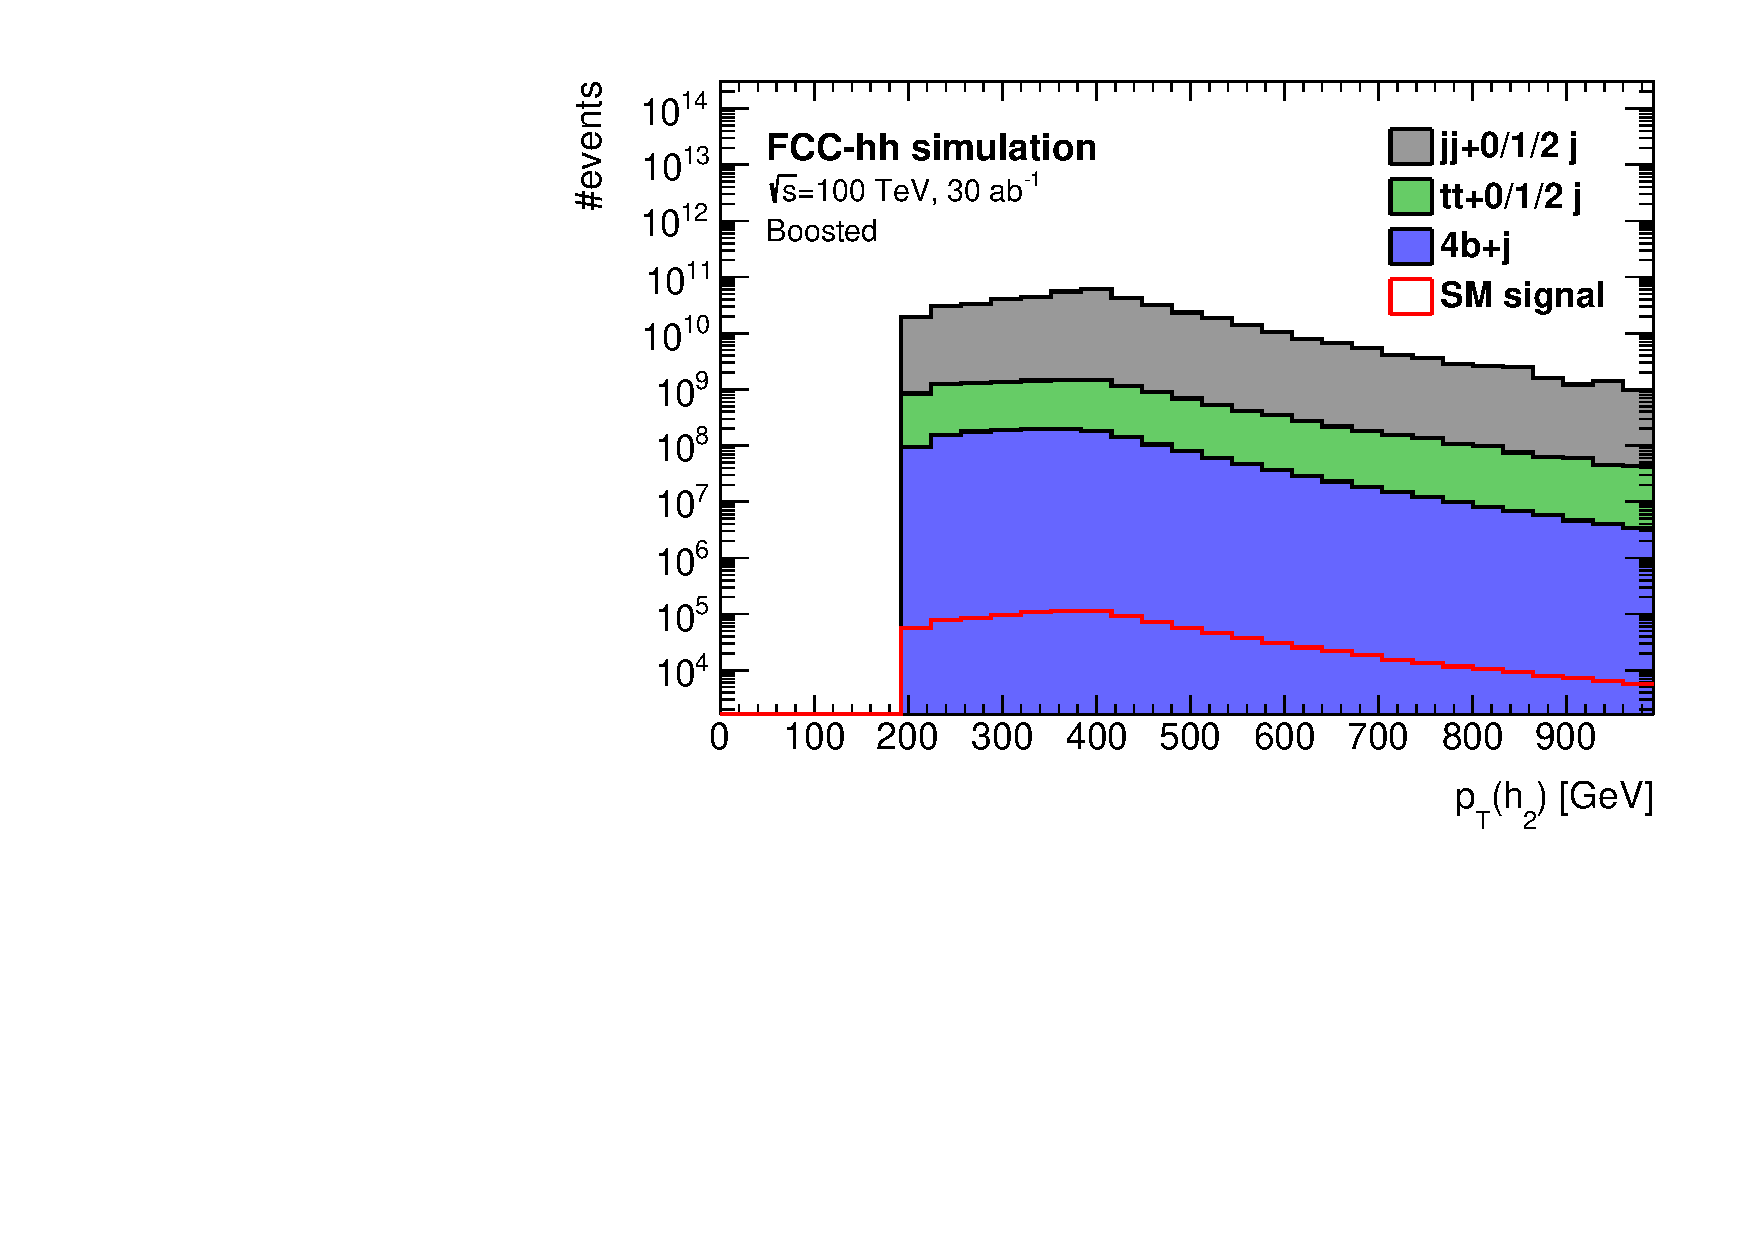
\includegraphics[trim={.65cm 0 0 0},clip,width=\linewidth]{./Figures/hist_h2_pt_stack.pdf}
		%\caption{oi}
		%\label{fig:h1_pt}
	\end{minipage}%
	\begin{minipage}{.5\textwidth}
		\centering
		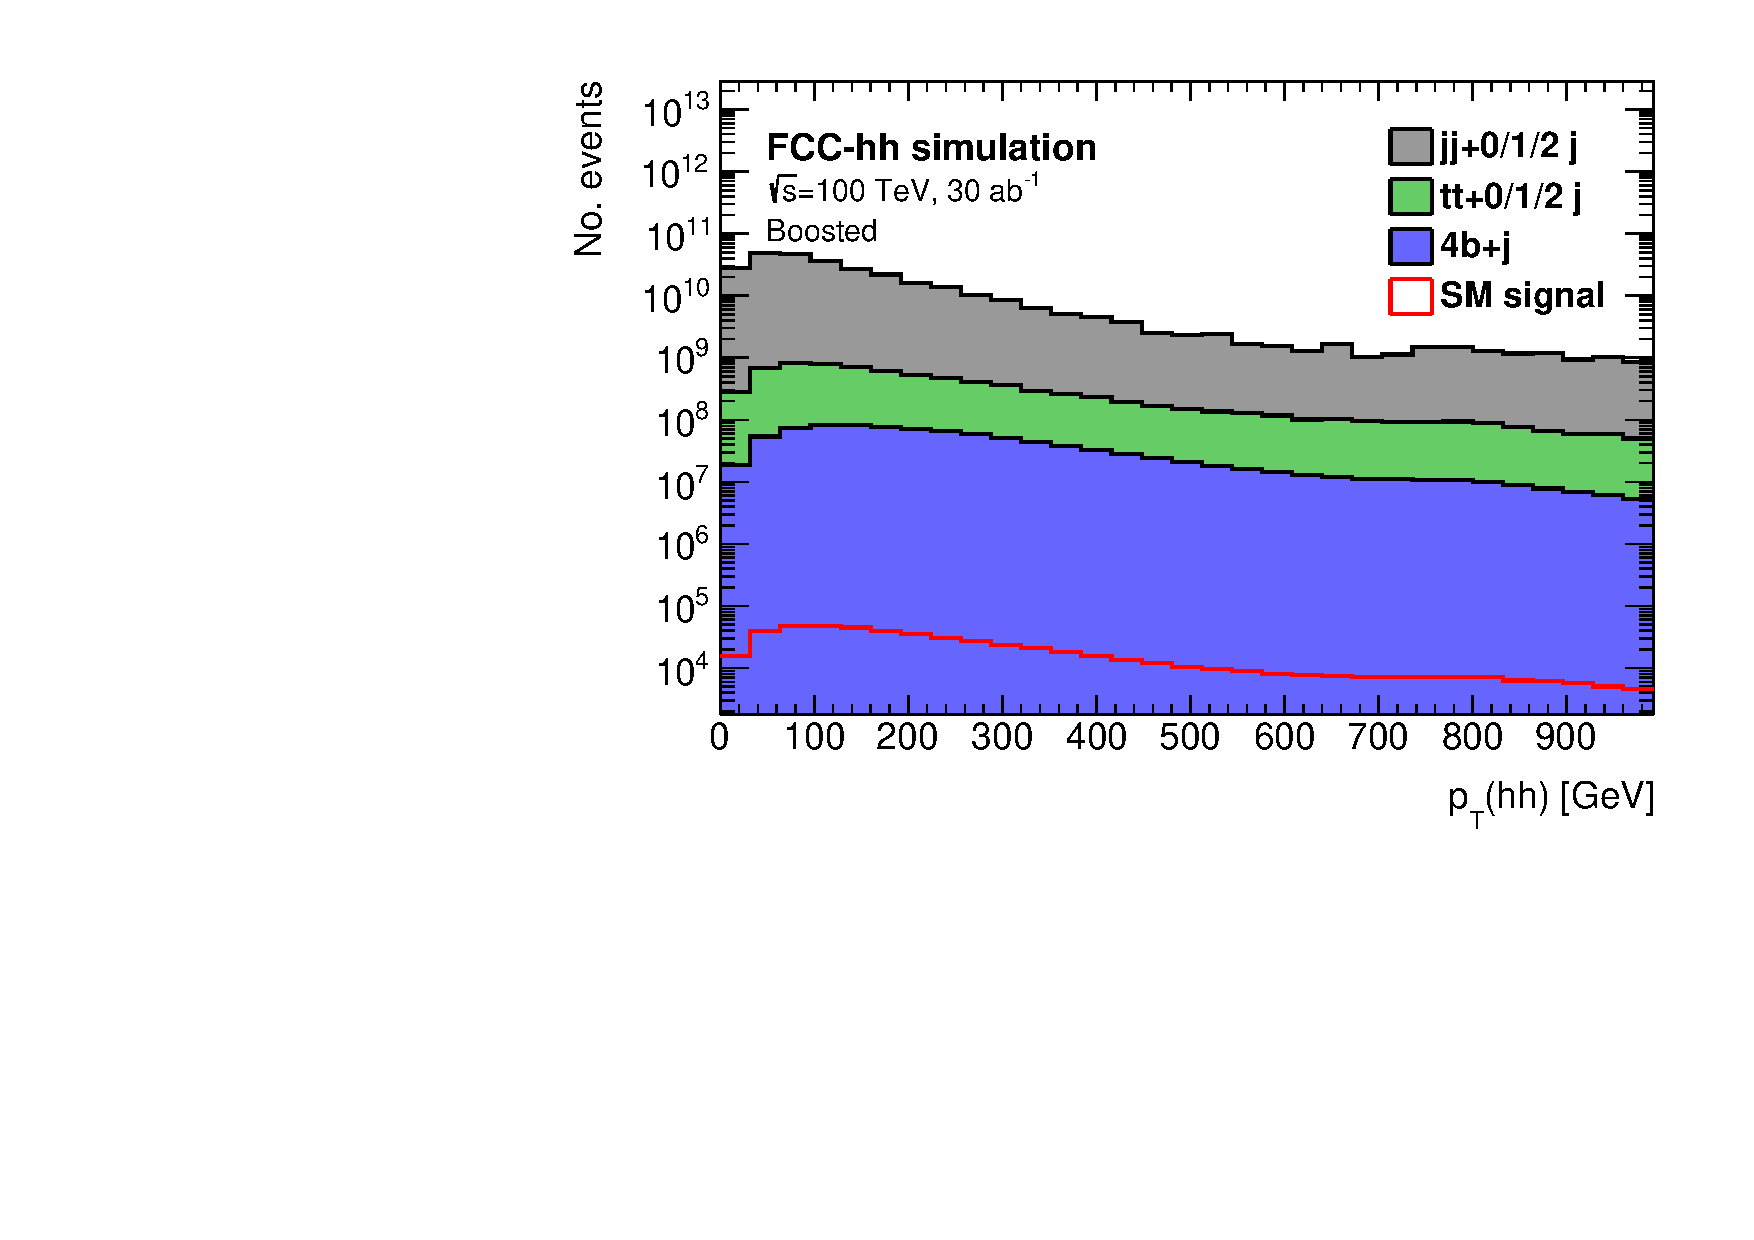
\includegraphics[trim={0 0 .65cm 0},clip,width=\linewidth]{./Figures/hist_hh_pt_stack.pdf}
		%\caption{oi}
		%\label{fig:h2_pt}
	\end{minipage}
	\label{fig:pt_stack}
	\caption{$p_T$ distributions for the sub leading Higgs candidate (left) and for the Higgs pair (right). The histograms are normalized to $\mathcal{L}=30~\text{ab}^{-1}$.}
\end{figure} 

\begin{figure}
	\centering
	\begin{minipage}{.5\textwidth}
		\centering
		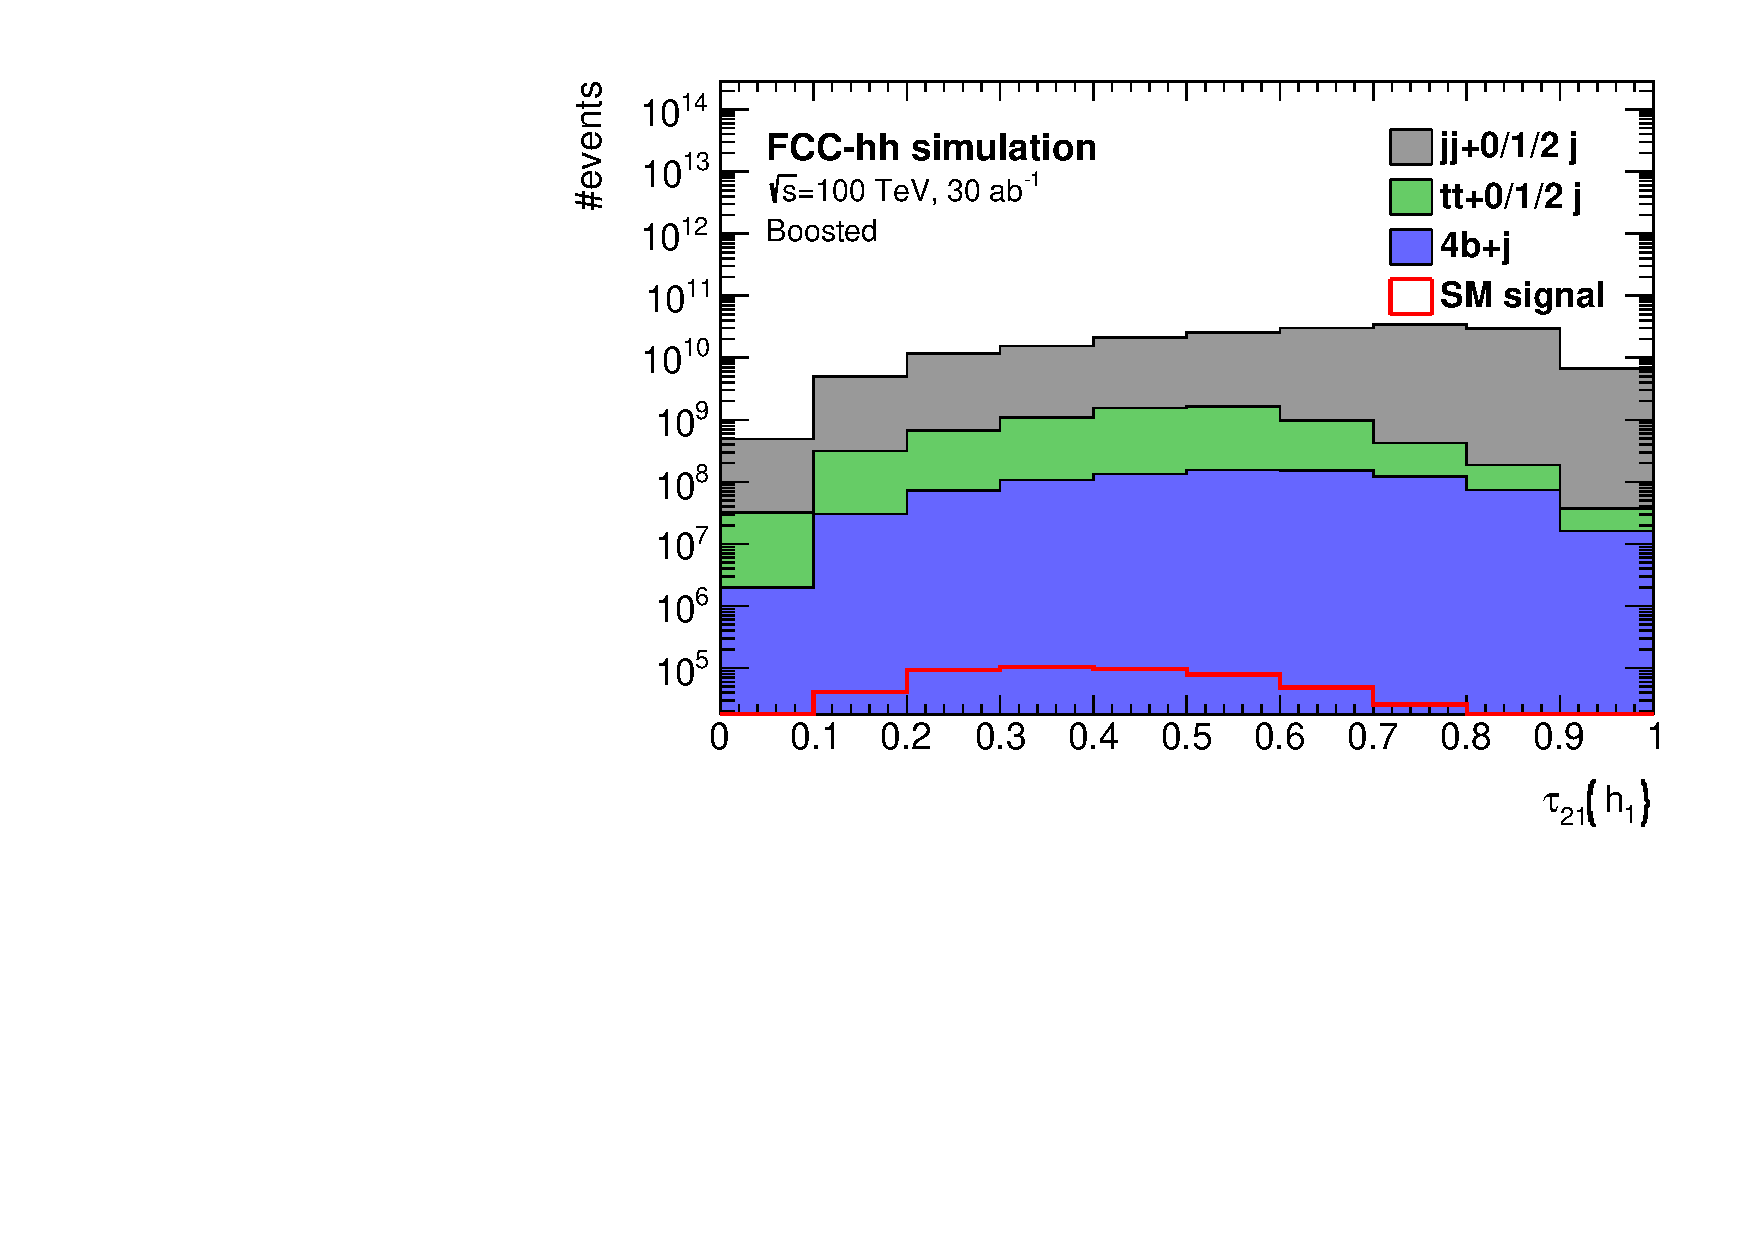
\includegraphics[trim={.65cm 0 0 0},clip,width=\linewidth]{./Figures/hist_h1_tau21_stack.pdf}
		%\caption{oi}
		%\label{fig:h1_pt}
	\end{minipage}%
	\begin{minipage}{.5\textwidth}
		\centering
		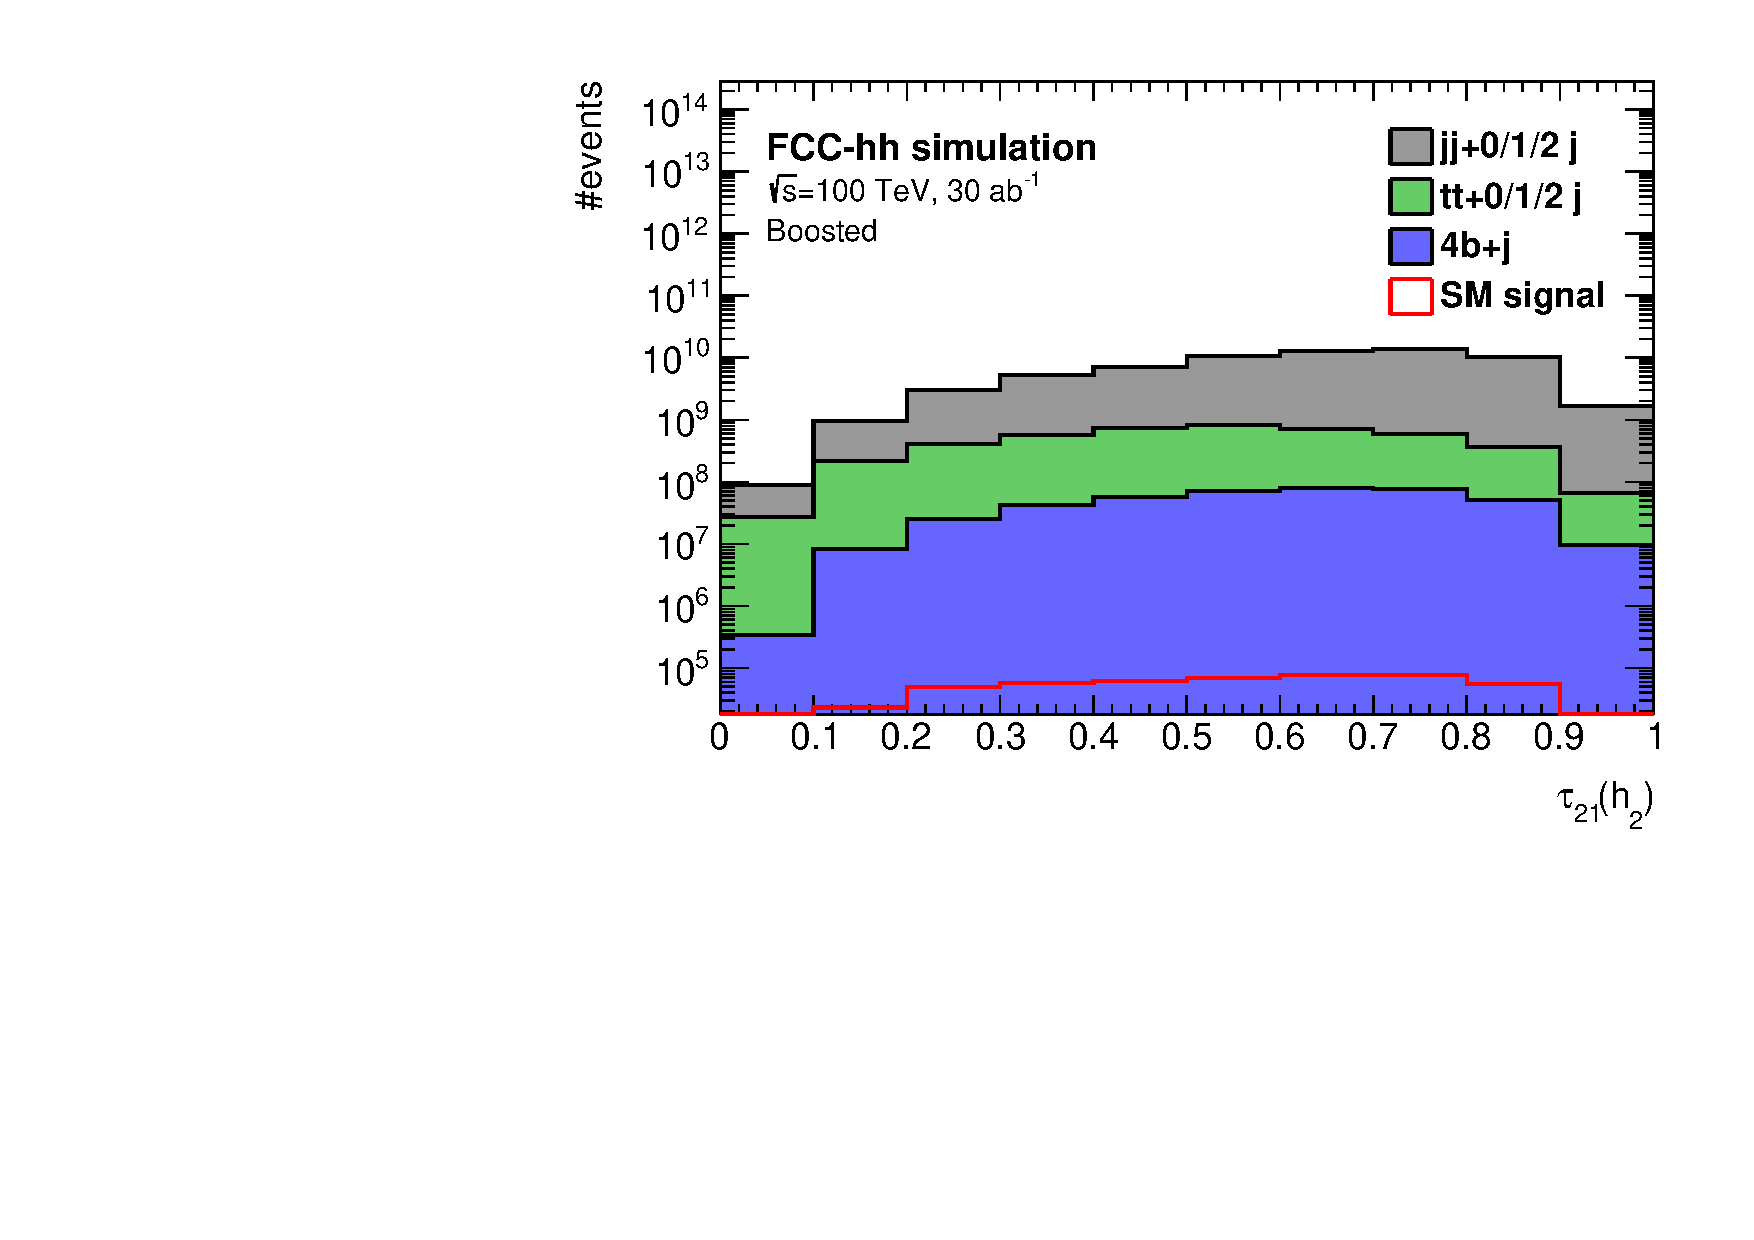
\includegraphics[trim={0 0 .65cm 0},clip,width=\linewidth]{./Figures/hist_h2_tau21_stack.pdf}
		%\caption{oi}
		%\label{fig:h2_pt}
	\end{minipage}
	\label{fig:sub_stack}
	\caption{Distributions of the $\tau_{21}$ variable for the leading (left) and sub leading (right) Higgs candidates. The histograms are normalized to $\mathcal{L}=30~\text{ab}^{-1}$.}
\end{figure} 

\begin{figure}
	\centering
	\begin{minipage}{.5\textwidth}
		\centering
		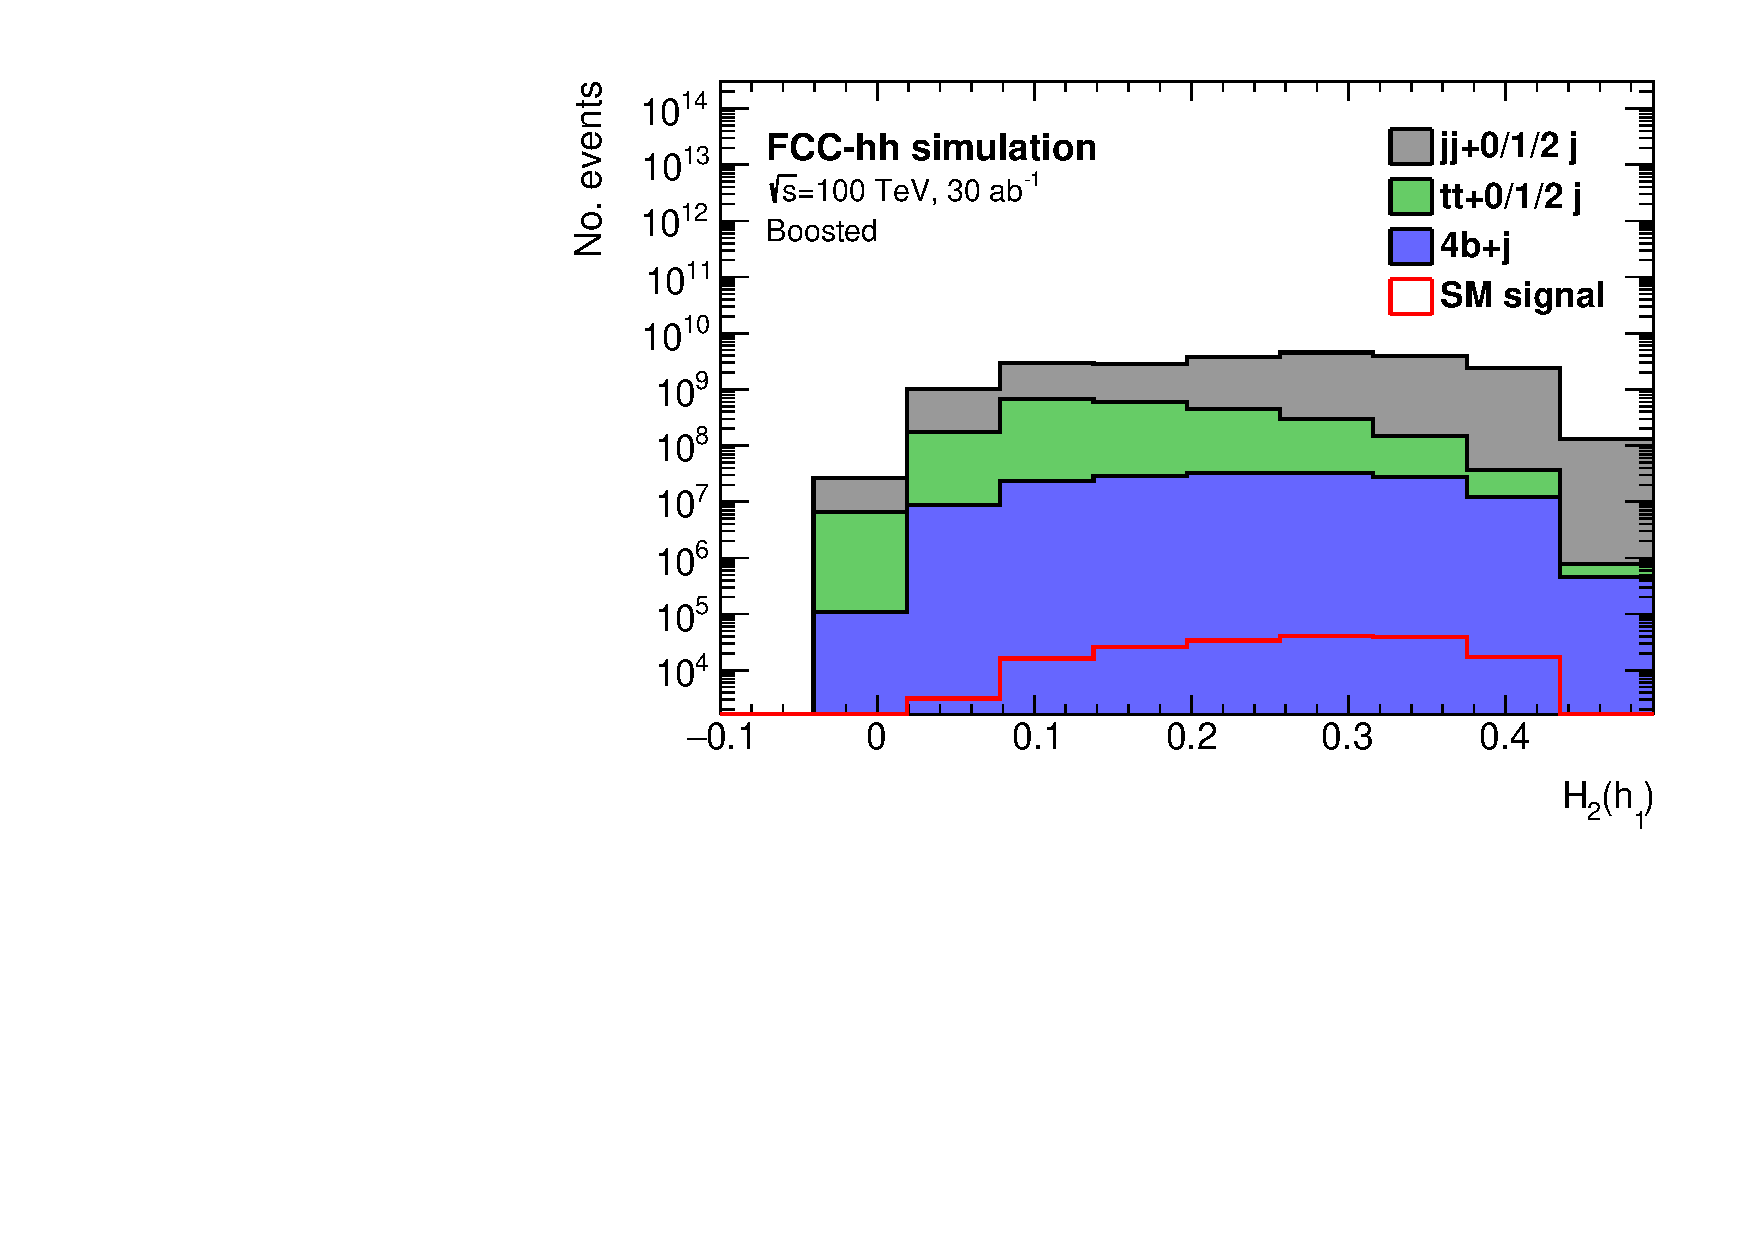
\includegraphics[trim={.65cm 0 0 0},clip,width=\linewidth]{./Figures/hist_h1_FW2_stack.pdf}
		%\caption{oi}
		%\label{fig:h1_pt}
	\end{minipage}%
	\begin{minipage}{.5\textwidth}
		\centering
		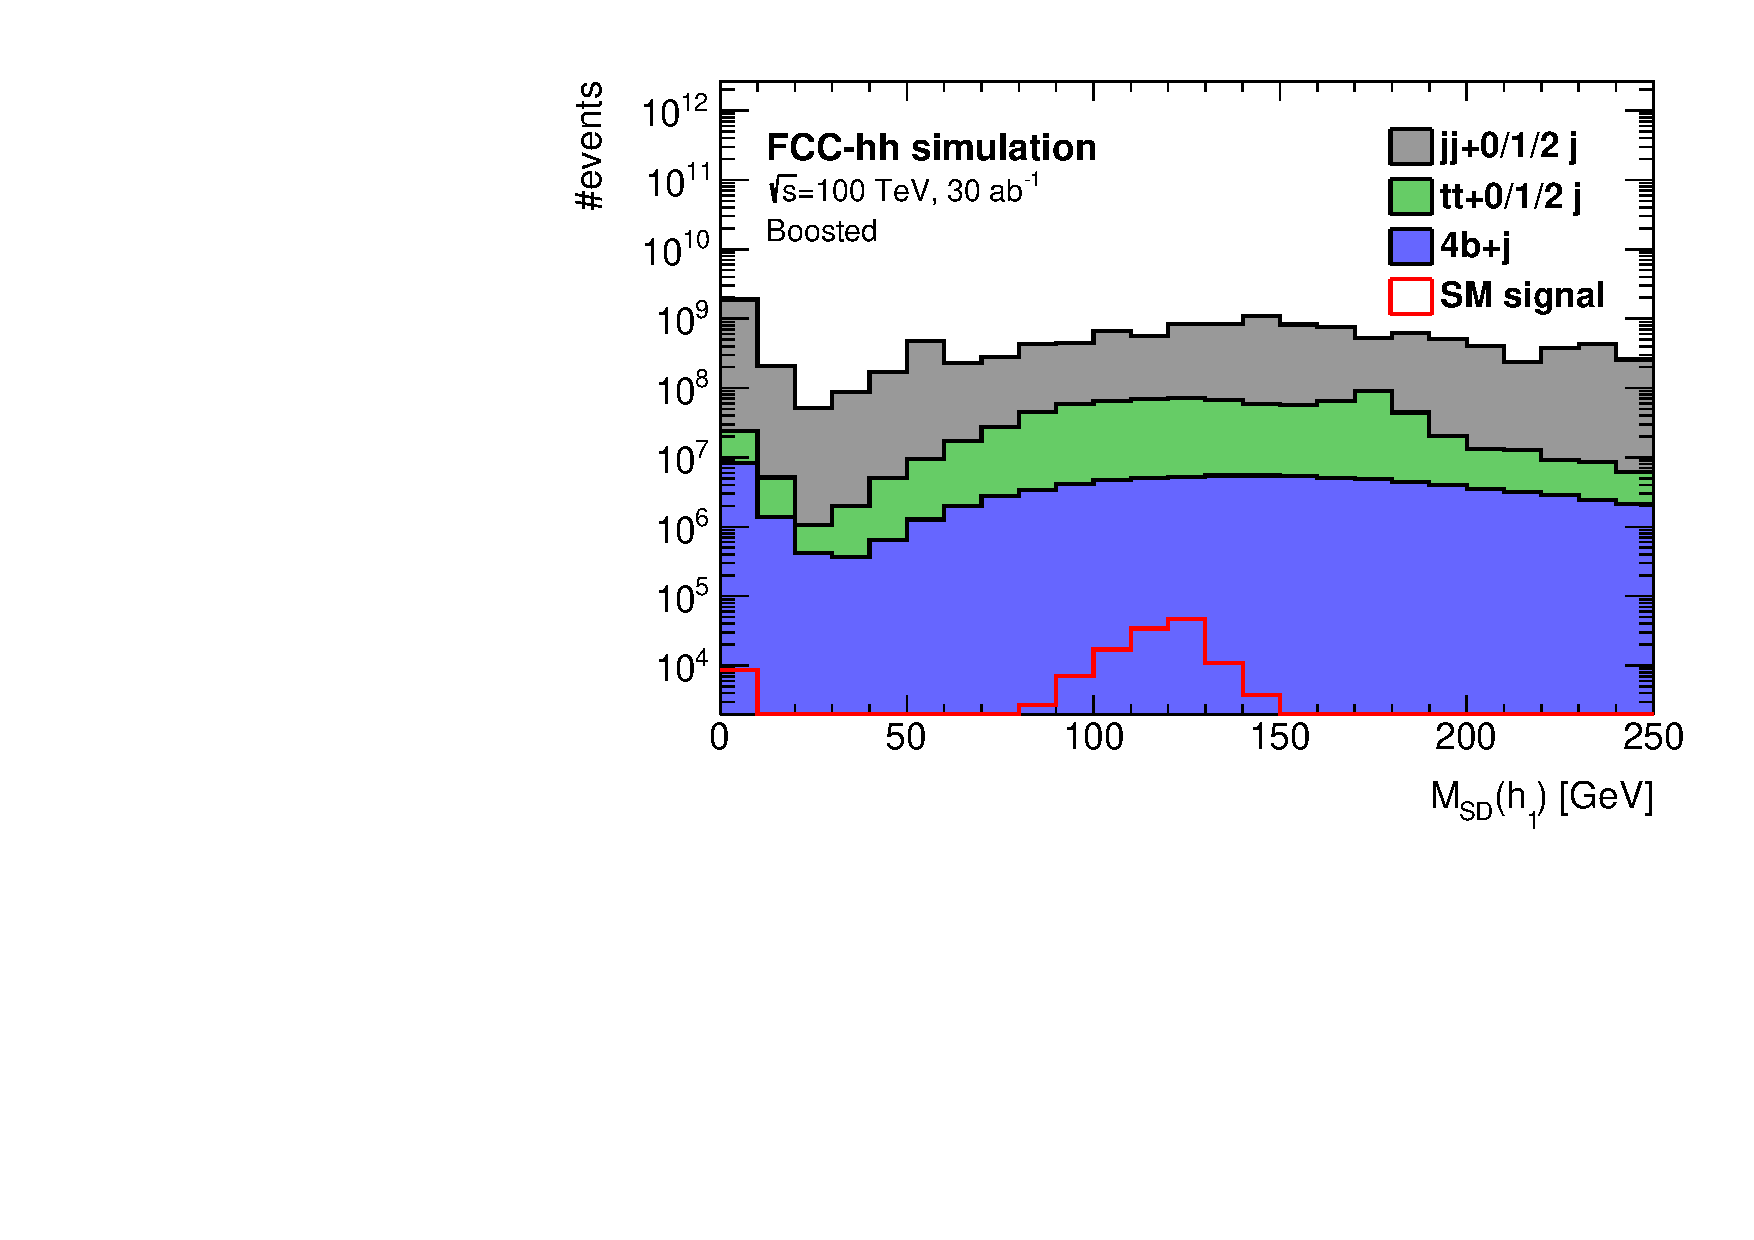
\includegraphics[trim={0 0 .65cm 0},clip,width=\linewidth]{./Figures/hist_h1_softdrop_M_stack.pdf}
		%\caption{oi}
		%\label{fig:h2_pt}
	\end{minipage}
	\label{fig:M_stack}
	\caption{$H_2$ variable for the leading Higgs candidate (left) and softdrop mass distribution for the leading Higgs candidate. The histograms are normalized to $\mathcal{L}=30~\text{ab}^{-1}$.}
\end{figure} 

\subsection{Optimization}

We explored different methods to optimize the baseline analysis in order to try to increase the achieved significance. 



TO INCLUDE:\\
- Mention study on correlations ? \\
- Optimization of cut-based analysis based on $S/\sqrt{B}$ plots \\
- MVA analysis ? 

%% ----------------------------------------------------------------------
%\subsection{Intermediate}
%\label{section:intermediate}
%
%- Event topology: one large R jet corresponding to the leading Higgs candidate and two small R jets corresponding to the b quarks of the sub leading Higgs candidate \\
%- Physics objects: fat jets (already described in previous section) and particle flow anti-kT R=0.4 jets \\
%- Selection criteria \\
%- Substructure variables: refer we (can)apply them to the fat jet \\
%- Optimization\\
%-------------------------------------------------------------------
% 
%This category targets events in which one of the Higgs bosons has a high Lorentz boost and therefore is reconstructed using a particle flow, anti-$k_T$ jet with $R=0.8$ (large-R jets). This is assumed to be the leading Higgs candidate. The sub leading Higgs boson, due to its relatively low $p_T$, can be fully reconstructed, meaning that each b quark is reconstructed using particle flow, anti-$k_T$ jets with $R=0.4$ (small-R jets). For the large-R jets the b-tagging is performed as described in the previous section. The small-R jets are b-tagged using Delphes default algorithm.
%
%\subsubsection{Event selection}
%
%We require exactly one large-R jet and at least two small-R jets. All jets have to be within $|\eta|<6$. The large-R jet is required to have $p_T>200$ GeV and the small-R jets are required to have $p_T>50$ GeV.
%% ----------------------------------------------------------------------
%\subsection{Resolved}
%\label{section:resolved}
%
%- Event topology: 4 small-R jets \\
%- Physics objects: small R jets already described in previous section \\
%- Selection criteria \\
%- Optimization (angular variables between b quarks, ...)\\
%-------------------------------------------------------------------
%
%This analysis category targets events in which the four b quarks can be reconstructed in four individual jets.
%
%The events are reconstructed using particle flow jets with $R=0.4$, clustered with the anti-$k_T$ algorithm. The b tagging is done using Delphes default algorithm.